\documentclass[12pt,letterpaper]{article}

\usepackage{amsmath, amsthm, amsfonts, amssymb}
\usepackage{microtype, parskip, graphicx}
\usepackage[comma,numbers,sort&compress]{natbib}
\usepackage[margin=1in]{geometry}
\usepackage{lineno}
\usepackage{longtable}
\usepackage{caption, subcaption, multirow, morefloats, rotating}
\usepackage{wrapfig}
\usepackage{hyperref}
\usepackage{threeparttable}

\frenchspacing


\newcommand{\beginsupplement}{
  \setcounter{table}{0}
  \renewcommand{\thetable}{S\arabic{table}}
  \setcounter{figure}{0}
  \renewcommand{\thefigure}{S\arabic{figure}}
  \setcounter{equation}{0}
  \renewcommand{\theequation}{S\arabic{equation}}
}



\title{How predictable is extinction? Forecasting species survival at million-year timescales}
\author{
  Smits, Peter\\
  %Department of Integrative Biology, University of California Berkeley\\
  \texttt{psmits@berkeley.edu} 
  \and
  Finnegan, Seth\\
  %Department of Integrative Biology, University of California Berkeley\\
  \texttt{sethf@berkeley.edu}
}

\begin{document}

\maketitle

\linenumbers{}
\modulolinenumbers[3]

\begin{abstract}
  One of the great promises of paleobiology is that by studying the past we can better predict the future. This promise is particularly pertinent given as risk assessments for some modern species could potentially be improved by examining past extinction patterns and by using paleontological records to establish geographic range and abundance trajectories on geological timescales. Any effort to assess future risk based on past extinctions and range trajectories must address two key questions:  (1) At a given timescale, are geographic range and extinction risk trajectories deterministic (past trends are likely to continue into the future) or Markovian (the future depends only on the present state)? (2) Given knowledge of past extinction/survival patterns and the present geographic ranges of extant taxa, how accurate are extinction risk predictions?  
  To address these questions we analyze the fossil record of Cenozoic planktonic microfossil taxa (foramanifera, radiolarians, diatoms, and calcareous nanoplankton). 
  We analyzed how survival probability changes over time as a function of species age, time of observation, current geographic range, most recent change in geographic range, global temperature average, and the lag of global temperature. 
  %Our best supported model includes the historical covariates, change in geographic range and lag of global temperature, which indicates that the past improves our estimates of the present and future. 
  Our results show that our best performing model has an approximately 78\% median probability of correctly ranking the relative extinction risk any two randomly selected species. 
  We have confidence that our conclusions about our ability to predict species extinction risk in the future with similar accuracy to when we predict species extinction risk in the past because our in-sample model performance measures are approximately equal to out-of-sample performance. 
  Including the historical covariates and allowing their effects to vary over time yields marginally better predictions than not including them. 
  However, the improvement in predictive power by including these historical covariates is modest at best, absent at worst, and ultimately reflects the extremely stochastic nature of species extinction. 
  %Finally, we find support for species' extinction risk increases with age, though the strength of this effect varies among taxonomic groups. 
  %This effect is most pronounced in forams and radiolarians, and less pronounced in diatoms and calcareous nanoplankton. 
  %The greatest source of variance in survival probability is the timing of observation. 
  %Importantly, this result means that the time of an observation is a greater source of variation in survival probability when compared to species age. 
  %We find that including information on a species' change in geographic range size on average improves our predictions of species survival at million-year timescales. 
  %The effect of change in geographic range is much smaller than the effect of current geographic range, and highly variable through time as the effect changes sign and there are times where there is little evidence for any effect of past geographic range. 
  These results imply that at million-year timescales geographic range trajectories are nearly Markovian, perhaps because the processes driving geographic range changes vary on substantially shorter timescales. 
  %The effect of change in geographic range on survival most likely stands for many interacting and unobserved processes which in-turn produce that species' geographic range and its affect on survival.  
  These results reflect the difficulty of estimating species extinction, and that while including historical covariates does improve model performance, that gain is very small. 
  The results of this study reinforce the importance of the promise of paleontology and using the past to predict the future.
\end{abstract}


\section{Introduction}

Being able to predict which species are more likely to go extinct than others is critical for making good conservation decisions to limit the impact of the current biodiversity crisis. We cannot know, however, we do not yet know which species are going to go extinct because this has not happened yet -- it is unobservable. We approach this this problem by analyzing the past in order to predict the future. The fossil record preserves past extinction events, allowing us to develop a predictive model of species extinction based on this record and the properties of the observed species, both extinct and extant \citep{Harnik2012,Finnegan2015}. By assessing the predictive performance of this model on unobserved data, we can quantify how precise our best estimates will be for future extinctions -- we ask the probability that, given two random species, we correctly rank their relative risks of extinction.

By studying how species vary in their extinction risk over time and we can assess which species are at greater risk under unobserved conditions. We know that a species' risk of extinction varies over time in both intensity (average rate) and selectivity (difference in risk between taxa) \citep{Payne2007,Payne2016,Ezard2011}. Species, after all, can go extinct at any ``moment'' and the relative risk of extinction exhibited by different taxonomic groups and how that risk varies over time is an important dynamic which shapes the rate and structure of extinction. What has not been evaluated is that as extinction intensity and selectivity change over time, how accurate are our assessments based on past events likely to be when applied to the future? By specifically including and modeling the temporal variation in extinction risk, we are able to improve our overall predictions because we incorporate and explicitly model differences between observations from across a range extinction intensities and selectivities.

By analyzing extinction and survival data from the fossil record, the hope is this can aide in predicting the extinction risk of extant species -- after all, the present must at some level be a function of the past. Past paleobiological studies of extinction have frequently focused on identifying and measuring the effect of various predictors on extinction risk \citep{Harnik2011,Smits2015,Peters2008,Payne2007,Harnik2012,Ezard2011,Foote2006} or on how to identify or measure these effects \citep{Alroy2010,Alroy2014,Alroy2001,Alroy2000,Alroy2000b,Foote2001}. This focus means that while we have a good understanding of which factors are strong and general determinates of extinction risk, we have less knowledge of how accurate or strong our predictions about the differences in extinction risk are. For example, while a predictor may be ``significant'' when comparing the odds of extinction risk between groups, the practical difference that predictor makes on prediction can be minimal \citep{ARM}. By including the kinds of biological and abiotic predictors that have been shown to affect differences in extinction risk, we can quantify their actual, as opposed to relative, effects on predictive performance.

A related question is if the changes to biotic or abiotic predictors, and not just their values, are similarly important factors for predicting extinction. For example, we know that a species' global geographic range changes over its duration \citep{Foote2007,Liow2010,Liow2007,Kiessling2013}. We also know that a species' geographic range size is a good predictor of differences extinction risk \citep{Payne2007,Jablonski2003,Jablonski2008,Jablonski2006}. This begs the question: how does a species' extinction risk change over its duration? While the phenomenon of species' geographic range change over time has been studied \citep{Foote2007,Liow2010,Liow2007,Kiessling2013}, the potential predictive impact of this change has been under-evaluated (but see \citet{Kiessling2013}). For example, does a species' extinction risk increase if that species decreased in global geographic range size over 1 million years? Here, we explicitly model and quantify the effects of changing geographic range as well as differences in global climate on how well we can predict species extinction. Similarly, we include species geologic age at time of observation as a potential predictor of extinction -- a factor that may or may not contribute to differences in species extinction risk over time \citep{Smits2015,Finnegan2008,Ezard2012,VanValen1973,Liow2011,Crampton2016}. Importantly, the inclusion of these ``historical'' predictors allows us to more fully evaluate the question of how much information about a species' past is necessary or useful when predicting a species' risk of extinction.

For this kind of exercise, we chose to analyze what is the longest continuous and best resolved fossil record -- that of skeletonized marine plantonic microorganisms from the Cenozoic such as Foraminifera, Radiolarians, Diatoms, and calcareous nannofossils (e.g. coccolithophores). This data is available through the Neptune database, an online repository of species occurrences obtained through the Deep Sea Drilling Program and the Ocean Drilling Project \citep{Lazarus1994,SpencerCervato1999}. This database provides abundant samples in space and time, a high degree of temporal resolution for the entirety of the Cenozoic, and has an internally consistent taxonomic identification strategy -- as close to ideal data for this analysis as possible. 

Rarely are we able to analyze long periods of geological time at fine resolutions -- below the 5-10 My scale. Due to substantial effort and the unique biology of the system, the microfossil provides us the unique opportunity to analyze ecological and evolutionary patterns at approximately million-year time scales. Typical ``exceptional'' fossil records tend to be of individual taxonomic groups and for rarely longer than 10 million years. The Neptune database records multiple phyla-scale taxonomic groups for over 60 million years, with incredible temporal resolution supported by the various age-models of the deep-sea cores the occurrences are recorded from -- there is no equivalent fossil record. By analyzing patterns of extinction and global occurrence at fine temporal scales, we can better elucidate how well we can predict species extinction at human-relevant scales.

%In particular, there have been multiple major climatic and oceanographic events, both short and protracted in duration, over the course of the Cenozoic. For example, the Paleocene-Eocene Thermal Maximum (PETM) was an geologically close-to instantaneous global warming event believed to have been caused by a massive injection of carbon into the atmosphere over a 20,000 year period which rapidly warmed and is associated with substantial changes to the global distribution of species CITATION. In contrast, the Eocene-Oligocene boundary is associated with a protracted global cooling event caused by the slow opening of Drake's passage and the development of the Antarctic ice sheet CITATION. These moments of large scale global change are inherently ``different,'' so predicting extinction before, during, and after these is important -- especially if those events are analogous to future climate change.

Being able to analyze over 60 million years of fossil occurrences allows to actually quantify how accurate our predictions are in general, but also how much variation there is in predictive accuracy over time and in many different environmental contexts. Specifically, we might expect that our model's predictive performance is best during prolonged periods of similar stress, such as the Eocene-Miocene transition \citep{Zachos2008} -- more samples from similar environments inherently improves future predictions in unobserved, but similar conditions. Alternatively, we would expect our model based predictions of extinction surrounding the Paleocene-Eocene Thermal Maximum may be less accurate because there are inherently fewer samples from the rapid climatic event \citep{Zachos2008}.



\section{Materials and Methods}

\subsection{Data Specifications}

We analyzed microfossil occurrence information which was downloaded from the Neptune Database \url{http://www.nsb-mfn-berlin.de/nannotax} \citep{Lazarus1994,SpencerCervato1999}. All occurrence information was downloaded for calcareous nannofossils, diatoms, foraminifera, and radiolarians -- these occurrences span the entire globe between 120 and 0 million years ago (Mya). This dataset of occurrences was then filtered to just those species which have their first occurrence at most 63 Mya. This choice means that our analysis avoids those taxa which survived the K/Pg boundary, those taxa which arose just after the K/Pg boundary, and means that our occurrence histories line up with the temperature time-series which was used as a predictor of extinction (discussed below).

All fossil occurrences were assigned to 1 My bins based on the estimated age of the fossil occurrence. Because the estimated ages of each occurrence is a product of core-specific age-models and can be overly precise, the hope is that by binning the data this smooths over the between-core heterogeneity and thus homogenizes our disparate data sources. The occurrence histories of each species were then given binary codes used to model the presence or extinction of those species. For every occurrence of a species, except the last, that species is considered to have survived and was marked with a 0. The last occurrence of that species is considered the bin in which the taxon has gone extinct -- and is assigned a 1. This protocol means that we are reading the fossil record ``as written,'' a practice that is potentially dangerous as it is a overconfident statement of preservation and may be shortening the actual duration of that species \citep{Alroy2010,Alroy2000b,Alroy2014,Foote1997,Foote1999a,Foote2001,Foote1996e,Lloyd2012b,Marshall1995,Wang2016}. However, this practice is common with marine microfossil data due to their exceptional preservation rate \citep{Ezard2013,Ezard2016,Ezard2011,Liow2010}. In fact, with marine microfossils collected from cores a bigger problem may be over extending the duration of a species due to mixing and smearing within the cores CITATIONS.

A taxon's geographic range was calculated for each of the 1 My bins in which it occurred. Geographic range was calculated as the maximum great circle distance on an ellipsoid (i.e. the Earth) between any two occurrences of that species; this measure is also called a geodesic. This distance was measured in kilometers. Geographic range was then log-plus-one transformed, and standardized by zero-centering the data and then dividing by the standard deviation of the distribution of geographic ranges. This standardization means that the analyzed values of geographic range had mean 0 and standard deviation 1. This standardization means that a regression coefficient associated with this covariate describes the change in extinction probability per change in standard deviation of geographic range, that coefficients associated with similarly standardized covariates will be directly comparable in magnitude, and that the interecpt term corresponds to the expected value of the outcome at when geographic range is its average value \citep{ARM}. Change in geographic range between observations was measured from the transformed and standardized geographic range values and not standardized seperately.

Temperature data used as covariates in this analysis are based on Magnesium/Calcium isotope ratios sourced from \citet{Cramer2011}. These elemental ratios are considered more accurate estimates of past global temperature when compared to the frequently used Oxygen isotope-based estimates; this is because Mg/Ca based estimates are not effected by ice-volume and fresh-water input (e.g. meteoric water) which can alter Oxygen isotope ratios without reflecting changes to the climate itself. This property is of particular importance for this analysis as polar ice-caps develop midway through the Cenozoic. Our data source, \citet{Cramer2011}, provides temperature estimates for every 0.1 My from 0 to 63 Mya. We binned these estimates into 1 My intervals as we did with the fossil occurrences. The temperature estimate for each 1 My interval was calculated as the mean of all estimates within that interval. Temperature was then transformed and standardized the in the same manner as geographic range (above). Difference in temperature between between observations was measured from the transformed and standardized temperature values and not standardized seperately.


%\begin{figure}[ht]
%  \centering
%  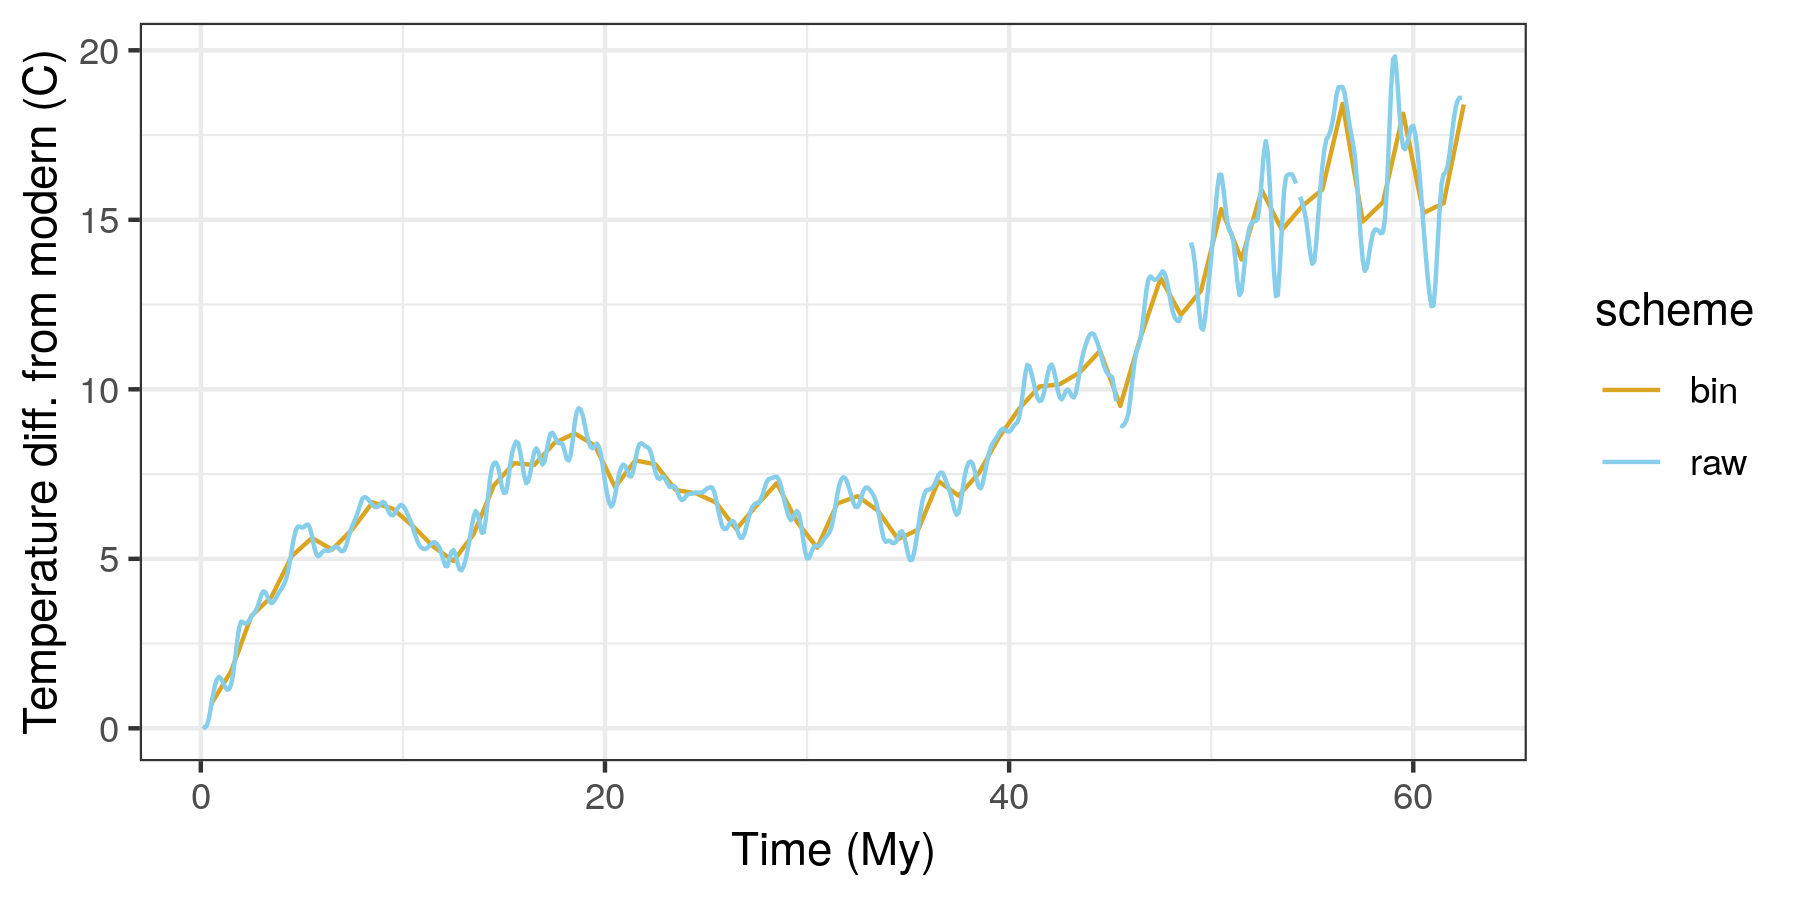
\includegraphics[width=\textwidth,height=0.5\textheight,keepaspectratio=true]{../results/figure/cramer_temp}
%  \caption{Comparison of initial temperature estimates from \citet{Cramer2011} (goldenrod) versus the binned values used in this analysis (blue). The initial values are for every 0.1 My while our bins are defined for every 1 My.}
%  \label{fig:temp_curve}
%\end{figure}


\subsection{Model Specifications}

We developed a discrete-time survival model to analyze our data in order to answer our question of how wee can we predict extinction risk at million year time scales. We considered four model variations: covariate effects are constant over time and none of our historical covariates are included (Model C), covariate effects are allowed to vary over time but we include none of our historical covariates (Model V), covariate effects are constant over time and our historical covariates are included (Model CP), covariate effects are allowed to vary over time and we include our historical covariates (Model VP). See Table \ref{tab:model_def} for further explanation of how these models differ from each other. For a complete description of the statistical model used in this analysis, please see Section \ref{sec:model_desc}. For a description of how our models were implemented, please see Section \ref{sec:model_est}.

\begin{table}[ht]
  \caption{Models and their definitions}
  \begin{threeparttable}
    {
      \def\arraystretch{1.5}
      \begin{tabular}{ l p{3cm} l l }
        Code & Description & Covariates & R Formula Syntax\tnote{a}\phantom{\textsuperscript{a}} \\
        \hline
        C & Constant effects, no historical cov. & \parbox[t]{0.25\textwidth}{Geographic range,\\temperature} & \parbox[t]{0.33\textwidth}{event\tnote{b}\phantom{\textsuperscript{b}} $\sim$ range\tnote{c}\phantom{\textsuperscript{c}} + temp\tnote{d}\phantom{\textsuperscript{d}} +\\(1 $|$ age\tnote{e}\phantom{\textsuperscript{e}}/phylum\tnote{f}\phantom{\textsuperscript{f}})} \\
        V & Varying effects, no historical cov. & \parbox[t]{0.25\textwidth}{Geographic range,\\temperature} & \parbox[t]{0.33\textwidth}{event $\sim$ range + temp +\\(1 + range + temp $|$ phylum) + (1 $|$ age/phylum)} \\ 
        CP & Constant effects, historical cov. & \parbox[t]{0.25\textwidth}{Geographic range,\\change in geographic range, temperature,\\previous temperature} & \parbox[t]{0.33\textwidth}{event $\sim$ range + range\_diff\tnote{g}\phantom{\textsuperscript{g}} +\\temp + temp\_lag\tnote{h}\phantom{\textsuperscript{h}} +\\(1 $|$ age/phylum)} \\
        VP & Varying effects, historical cov. & \parbox[t]{0.25\textwidth}{Geographic range,\\change in geographic range, temperature,\\previous temperature} & \parbox[t]{0.33\textwidth}{event $\sim$ range + range\_diff +\\temp + temp\_lag +\\(1 + range + range\_diff +\\temp + temp\_lag $|$ phylum) +\\(1 $|$ age/phylum)} \\
        \hline
      \end{tabular}
    }
    \begin{tablenotes}
    \item[a] See Equation \ref{eq:model} for full statistical model definition.
    \item[b] Species observation where 1 if time of last observation, otherwise 0.
    \item[c] Species geographic range in log km\(^2\). Mean centered, scaled to sd = 1.
    \item[d] Global temperature in degrees C. Mean centered, scaled to sd = 1.
    \item[e] Species are at observation in millions of years.
    \item[f] Taxonomic group of species (i.e. Foraminifera, Diatoms, Radiolarians, Calcaeous nannoplankton).
    \item[g] Change in geographic range since last observation.
    \item[h] Temperature at previous observation.
    \end{tablenotes}
  \end{threeparttable}
  \label{tab:model_def}
\end{table}


\subsection{Model adequacy}

We are interested in model adequacy and performance into two contexts: in-sample and out-of-sample predictive performance. ``In-sample'' means we are estimating how well our model predicts our observed data given that the model was fit to the entire dataset; this is a posterior predictive check in that we are comparing the posterior predictive distribution to our observed data. ``Out-of-sample'' is defined below.

Relative and absolute model adequacy of the four variant models was compared using the area under the receiver operating characteristic curve or AUC \citep{Fawcett2006,Mason2002}. This measure is commonly used in classification problems as it has the desirable characteristic of comparing the model's true positive rate with its false positive rate, as opposed to accuracy which only considers the count of true positives. AUC ranges between 0.5 and 1, with 0.5 indicating no improvement in performance from random and 1 indicating perfect performance. AUC can be interpreted as the probability that our model correctly ranks the relative extinction risks of any two randomly selected species \citep{Fawcett2006,Mason2002}.

The differences in in-sample predictive performance between the models was visualized in multiple ways: whole data set by model, taxonomic group by model, model performance over time, and model performance by taxonomic groups over time. These comparisons demonstrate the relative and absolute adequacy of the models in describing the dataset they were fit to.

We are particularly interested in understanding how well our model predicts species extinction given new, future data (out-of-sample data). To do this, we estimated average out-of-sample predictive error using 5-fold time-series cross-validation. For time-series data, the folds (data partitions) are approximately equal segments of time. The model is fit to the first fold and the posterior estimates are used to predict the states of the observations in the second fold, then the model is fit to the first and second fold and the posterior states are used to estimate the states from the third fold, and so on with increasingly large numbers of folds used for fitting a model to predict the states from the subsequent fold. With 63 time points, each of the five folds represents approximately 13 time points. Keep in mind, however, that each time point corresponds to many (100-1000) individual observations.


See our code repository LINK for full code details. Our code uses ``tidyverse'' tools such as \texttt{dplyr} \citep{dplyr}, \texttt{purr} \citep{purrr}, and \texttt{tidybayes} \citep{tidybayes}, thus some familiarity with that package ecosystem is necessary to fully comprehend how we've processed our data and results.


\section{Results}

% ROC model comparison
\begin{figure}[ht]
  \begin{subfigure}[ht]{0.45\textwidth}
    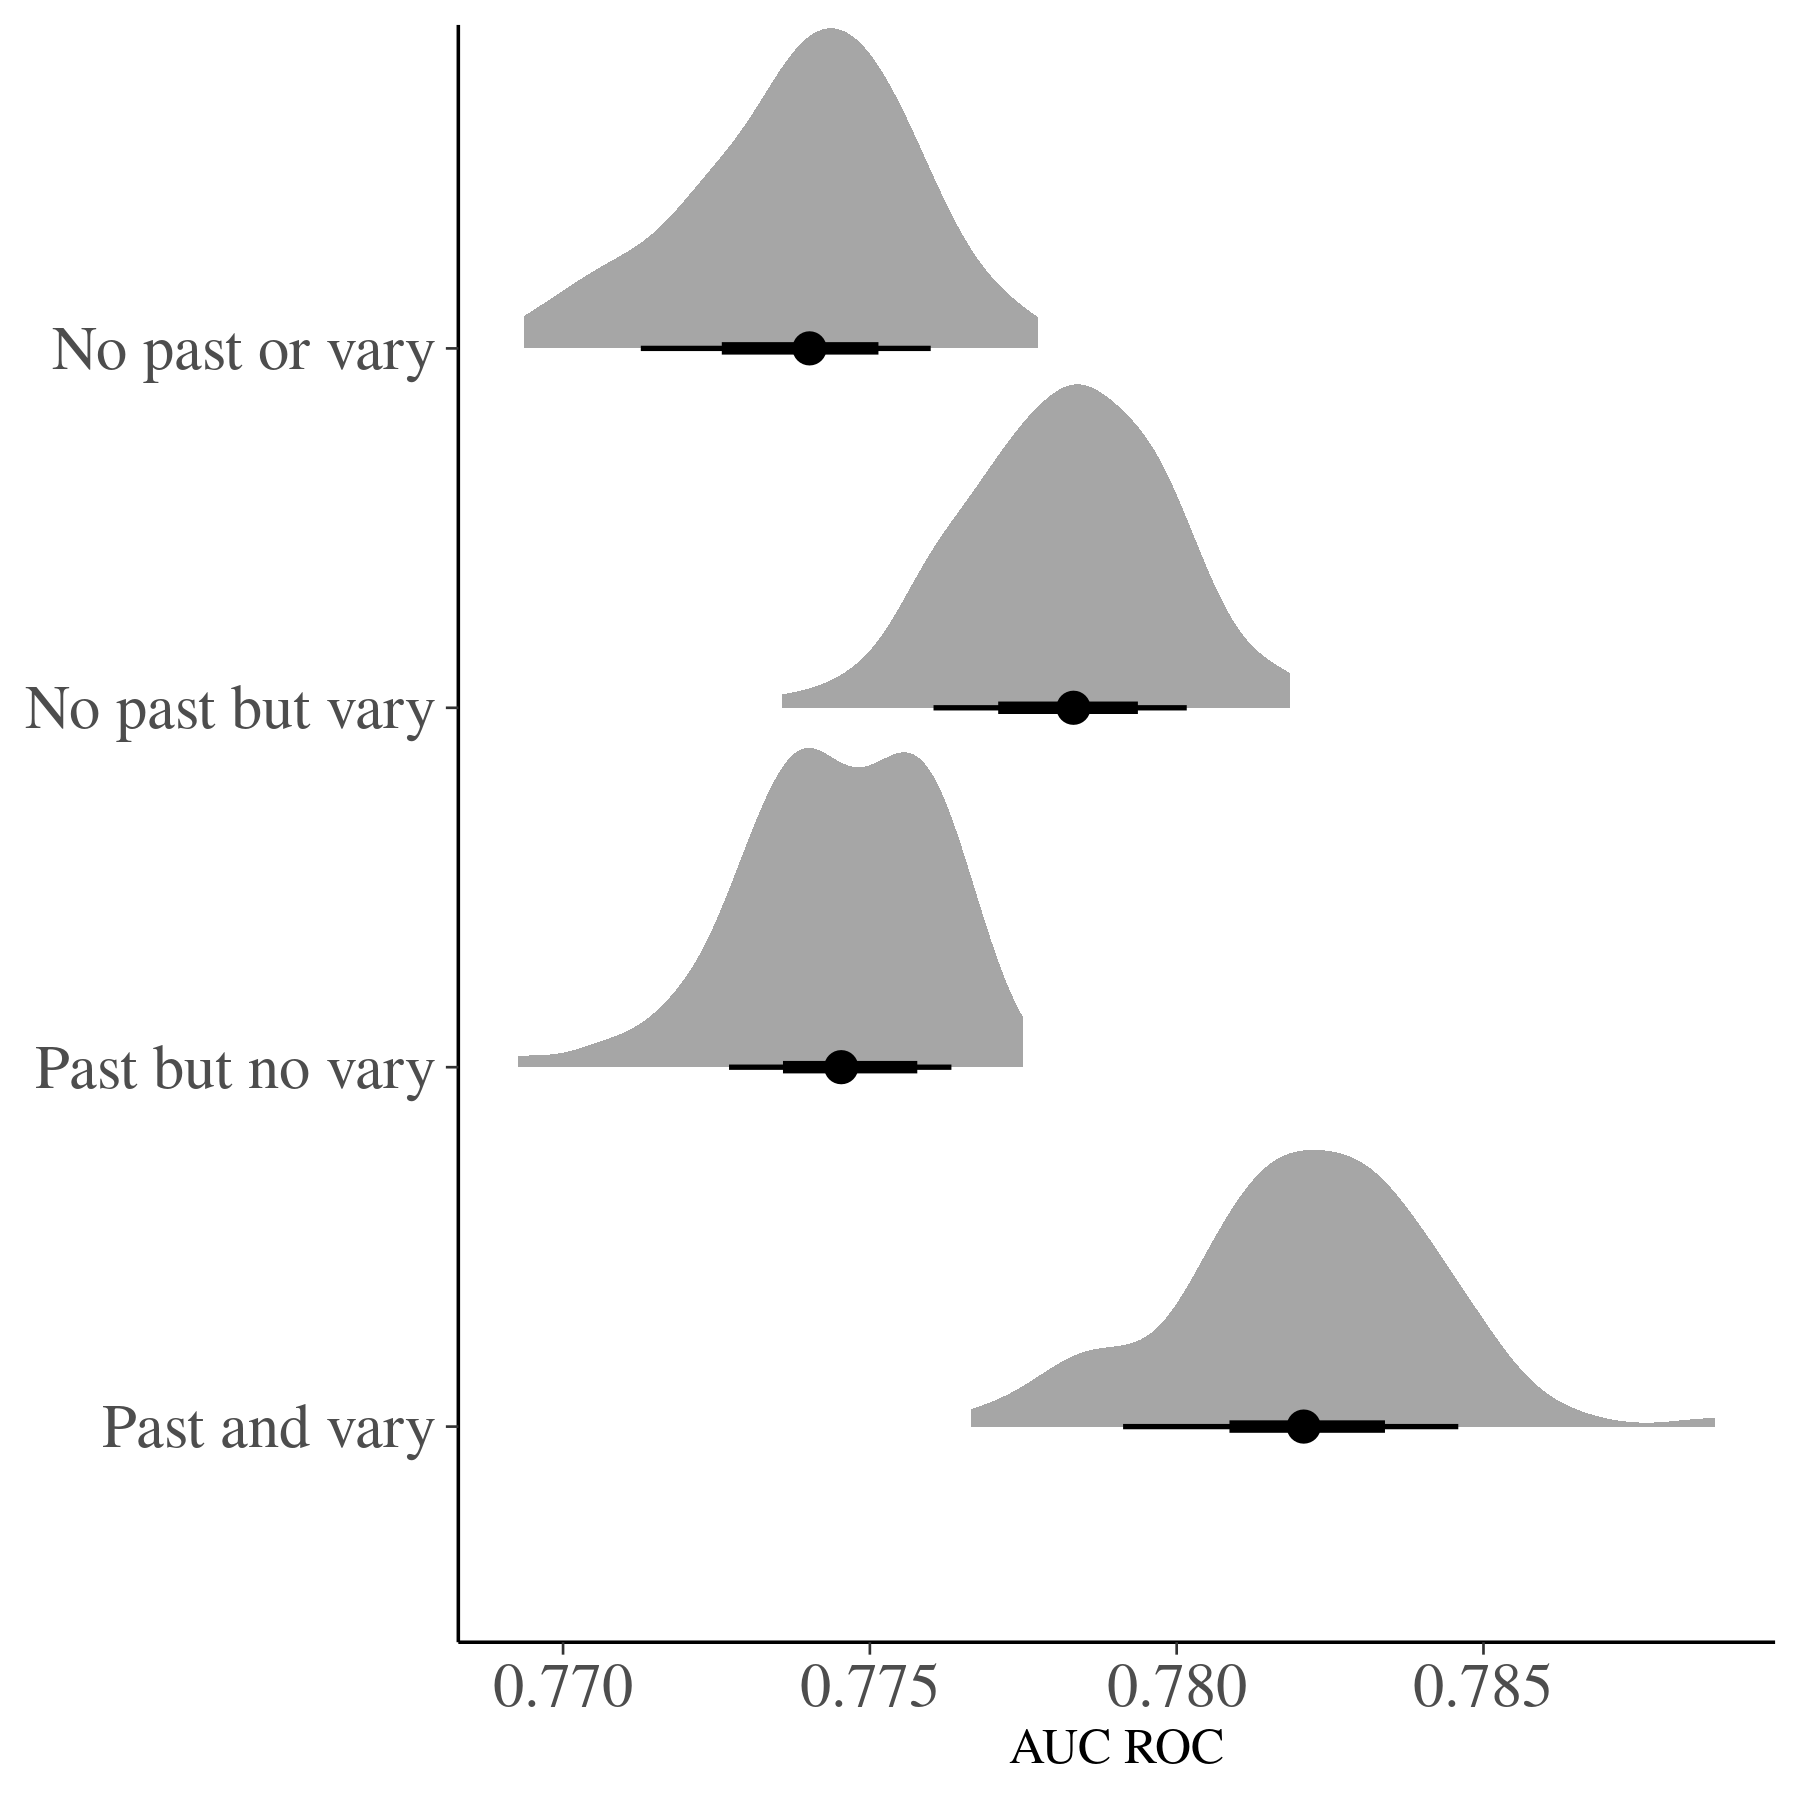
\includegraphics[width=\textwidth,height=0.5\textheight,keepaspectratio=true]{../results/figure/auc_hist_full}
    \caption{In-sample}
    \label{fig:auc_hist}
  \end{subfigure}
  \begin{subfigure}[ht]{0.45\textwidth}
    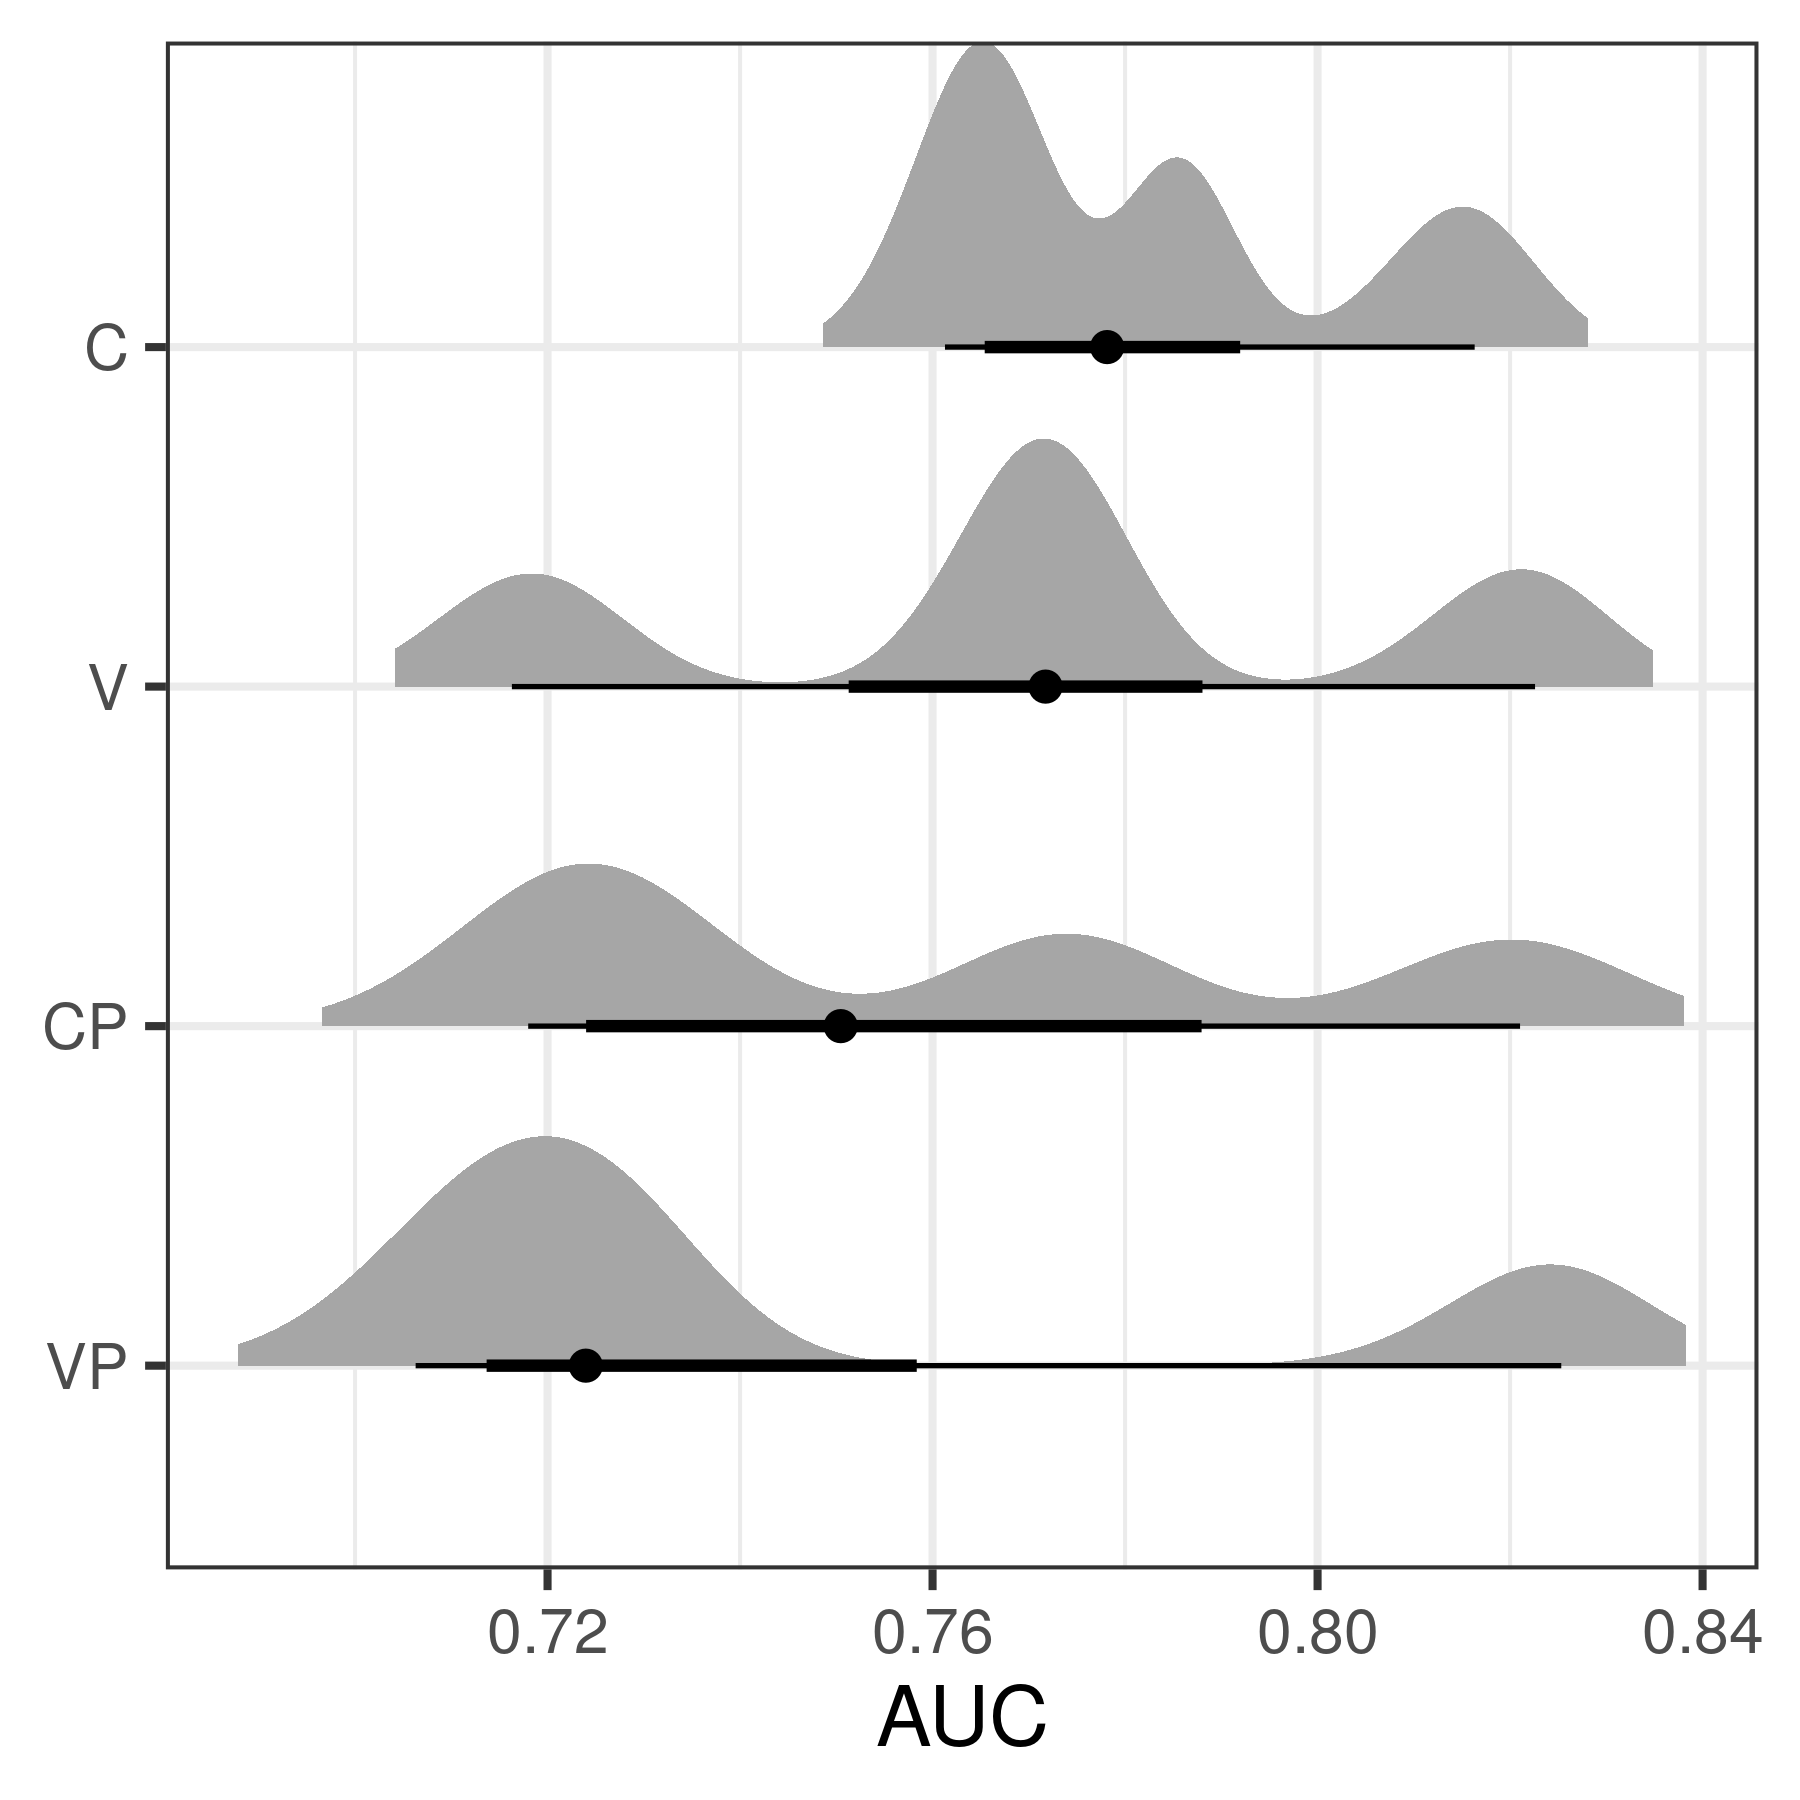
\includegraphics[width=\textwidth,height=0.5\textheight,keepaspectratio=true]{../results/figure/fold_auc_full}
    \caption{Out-of-sample}
    \label{fig:fold_auc}
  \end{subfigure}
  \caption{In-sample (\ref{fig:auc_hist}) and out-of-sample (\ref{fig:fold_auc}) AUC estimates for each of our four models. These estimates are calculated from the models posterior predictive distribution or from predictions made to new data, respectively. Models with a higher AUC values indicate better performance over models with lower AUC values. AUC is bounded between 0.5 and 1. See Table \ref{tab:model_def} for a description of each of the four models.}
  \label{fig:auc_compare}
\end{figure}

\subsection{Model adequacy}

The in-sample model comparisons are for determining their relative adequacy, or a model's ability to represent the data it was fit to. Comparison between the posterior predictive estimates of in-sample AUC for each of the four models demonstrates that, overall, all of the models have approximately equal in-sample performance (Fig. \ref{fig:auc_hist}). The parameter rich model VP has the greatest median in-sample AUC when compared to the other three models, but there is substantial overlap in their posterior distributions. Additionally, while our parameter rich model VP is possibly the most adequately performing model, the difference or improvement to performance is minimal at best -- all four models have approximately equal in-sample AUC posterior distributions. All of the in-sample AUC estimates from our models are concentrated around an AUC of 0.77 which is interpreted as ``fine but not good'' performance. It is then hard to conclude that there is one ``best'' model which we can rely upon. 

%When the posterior predictive distributions of the in-sample AUC estimates are presented over time, the similarity in adequacy between the models becomes more apparent (Fig. \ref{fig:auc_ts}). There are few major or obvious differences in model adequacy between the four models.
%% ROC model comparison time series
%\begin{figure}[ht]
%  \centering
%  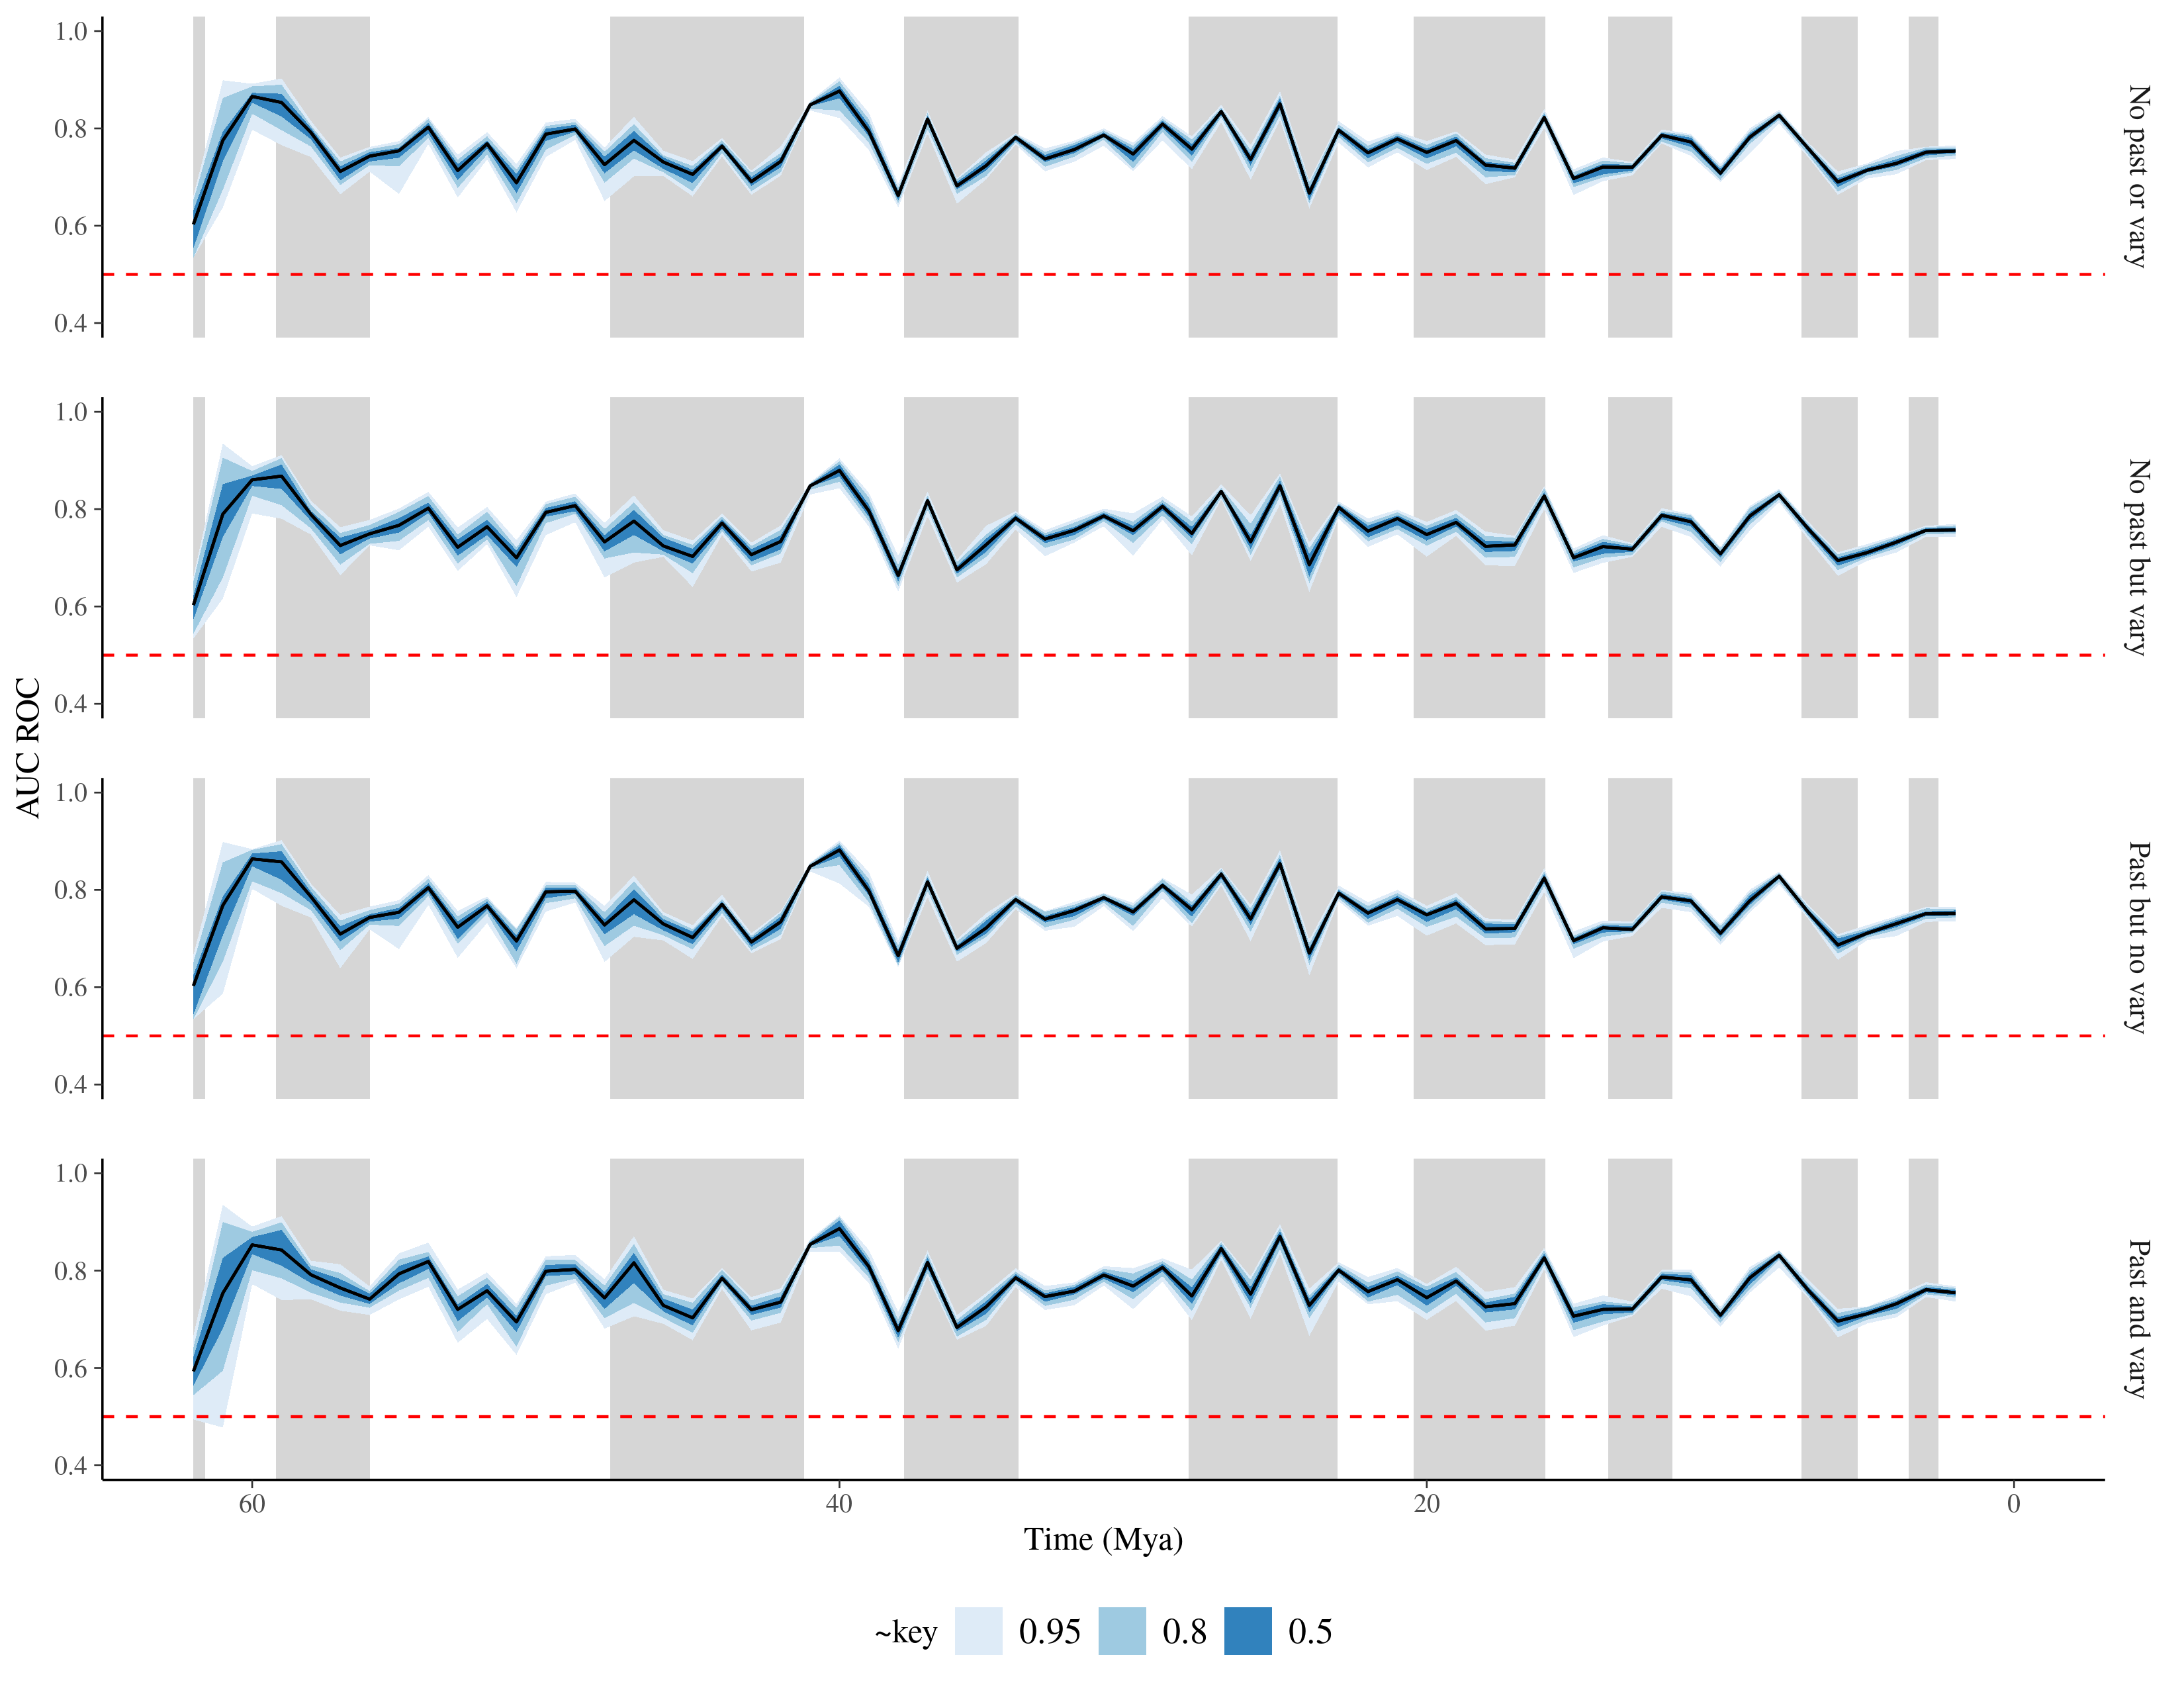
\includegraphics[width=\textwidth,height=0.5\textheight,keepaspectratio=true]{../results/figure/auc_ts_full}
%  \caption{Comparison between the posterior predictive AUC estimates for each of the time intervals for each of the four models. These estimates are reflections of each model's fit to the various time intervals. The red line corresponds to the median AUC value, while the envelopes correspond to multiple credible intervals as indicated in the legend. In all cases, higher AUC values indicate greater predictive performance versus lower AUC values.}
%  \label{fig:auc_ts}
%\end{figure}


%When the posterior predictive distributions of the in-sample AUC estimates are presented by taxonomic group, some heterogeneity in model adequacy is revealed (Fig. \ref{fig:auc_taxon}). While in all cases the model with the highest average in-sample AUC is the parameter-rich ``past and vary'' model, the amount of difference between the models varies by taxonomic group in ways not observable from the pooled estimates (Fig. \ref{fig:auc_hist}). For example, the difference between the ``past and vary'' model and the others is more pronouced for Calcareous nannoplankton and Dinoflagellates, and smaller for the Foraminifera and Radiolaria. 
%\begin{figure}[ht]
%  \centering
%  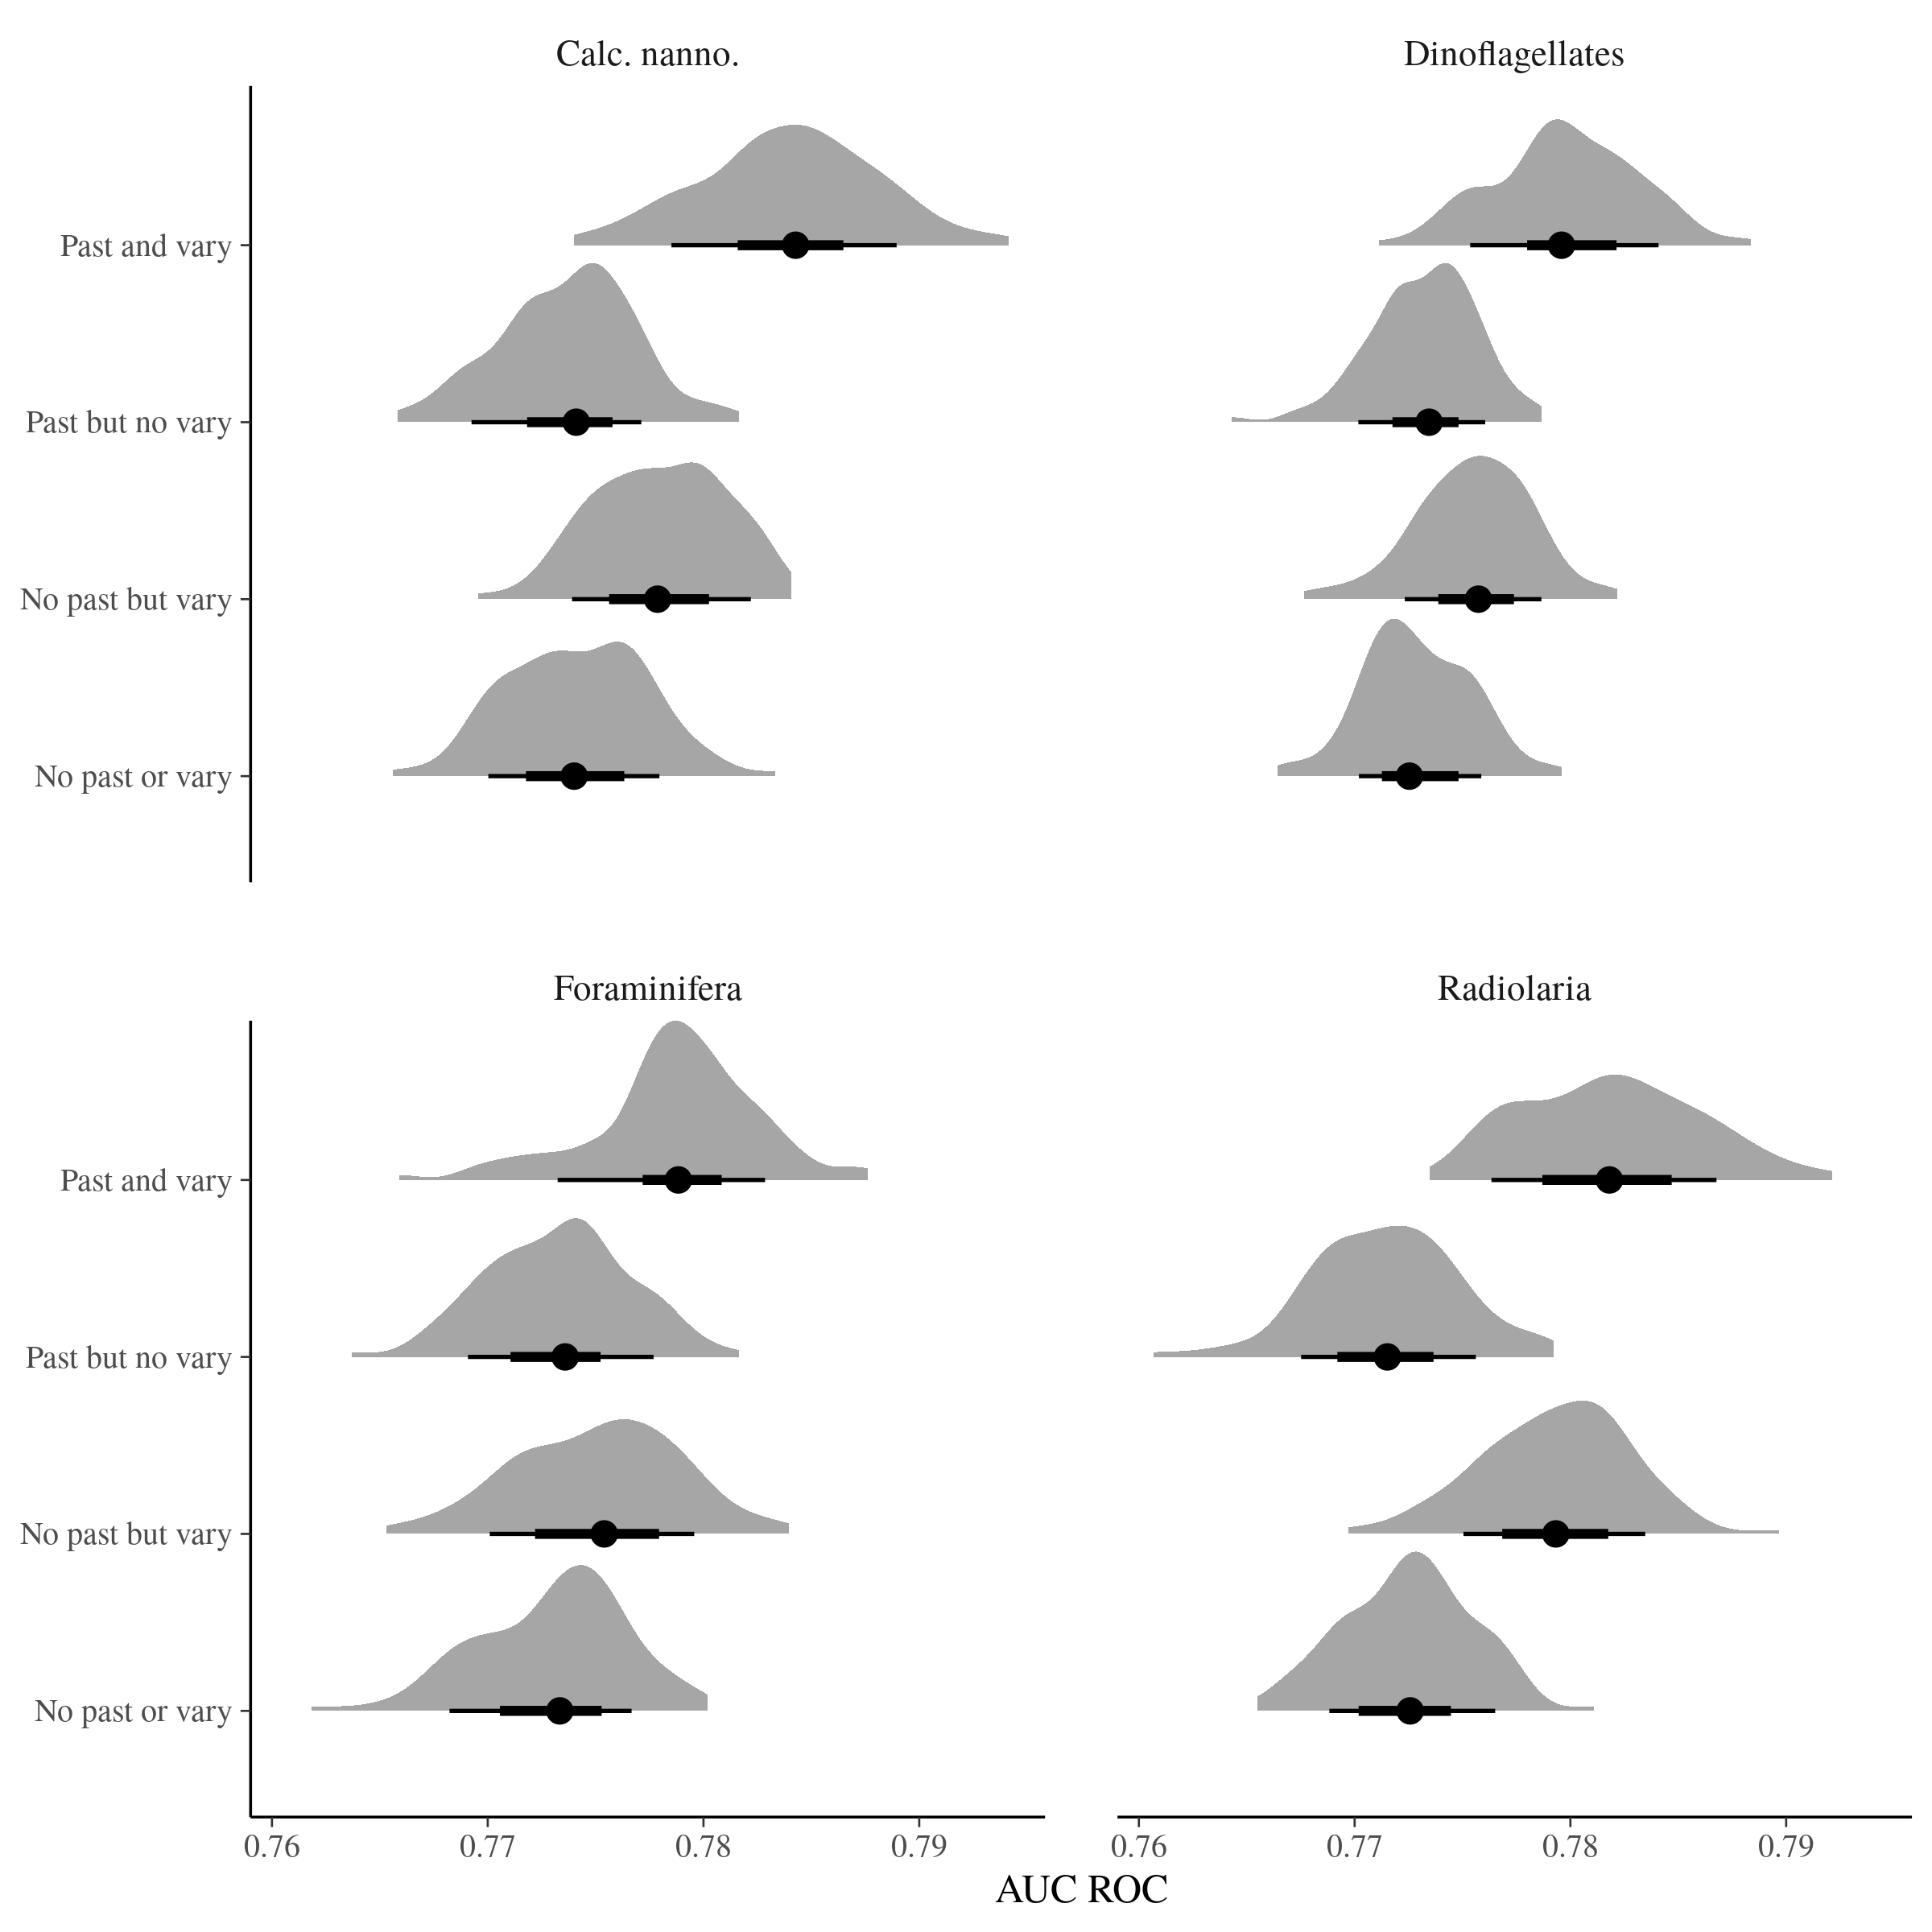
\includegraphics[width=\textwidth,height=0.5\textheight,keepaspectratio=true]{../results/figure/auc_taxon_full}
%  \caption{Comparison of posterior predictive AUC estimates for each of the four models, arranged by taxonomic group. These estimates reflect each model's fit to the various taxonomic groups present in this analysis. The densities reflect the posterior distribution of the estimates, and below each density is marked the median AUC value along with the 50\% and 80\% credible intervals. In all cases, higher AUC values indicate greater predictive performance versus lower AUC values.}
%  \label{fig:auc_taxon}
%\end{figure}


For many taxon/model combinations there are one or more time periods where posterior predictive in-sample AUC has a median value less than or equal to 0.5 -- AUC value of 0.5 indicates that the model's predictions are no better than random (Fig. \ref{fig:auc_taxon_time}). However, this pattern is absent for the posterior predictive distribution of Foraminfera and Radiolaria for the VP model. Additionally, these periods of low model performance are rarer for the posterior predictive distribution of the VP model for calcareous nannoplankton and Dinoflagellates when compared to the other three models.
\begin{figure}[ht]
  \centering
  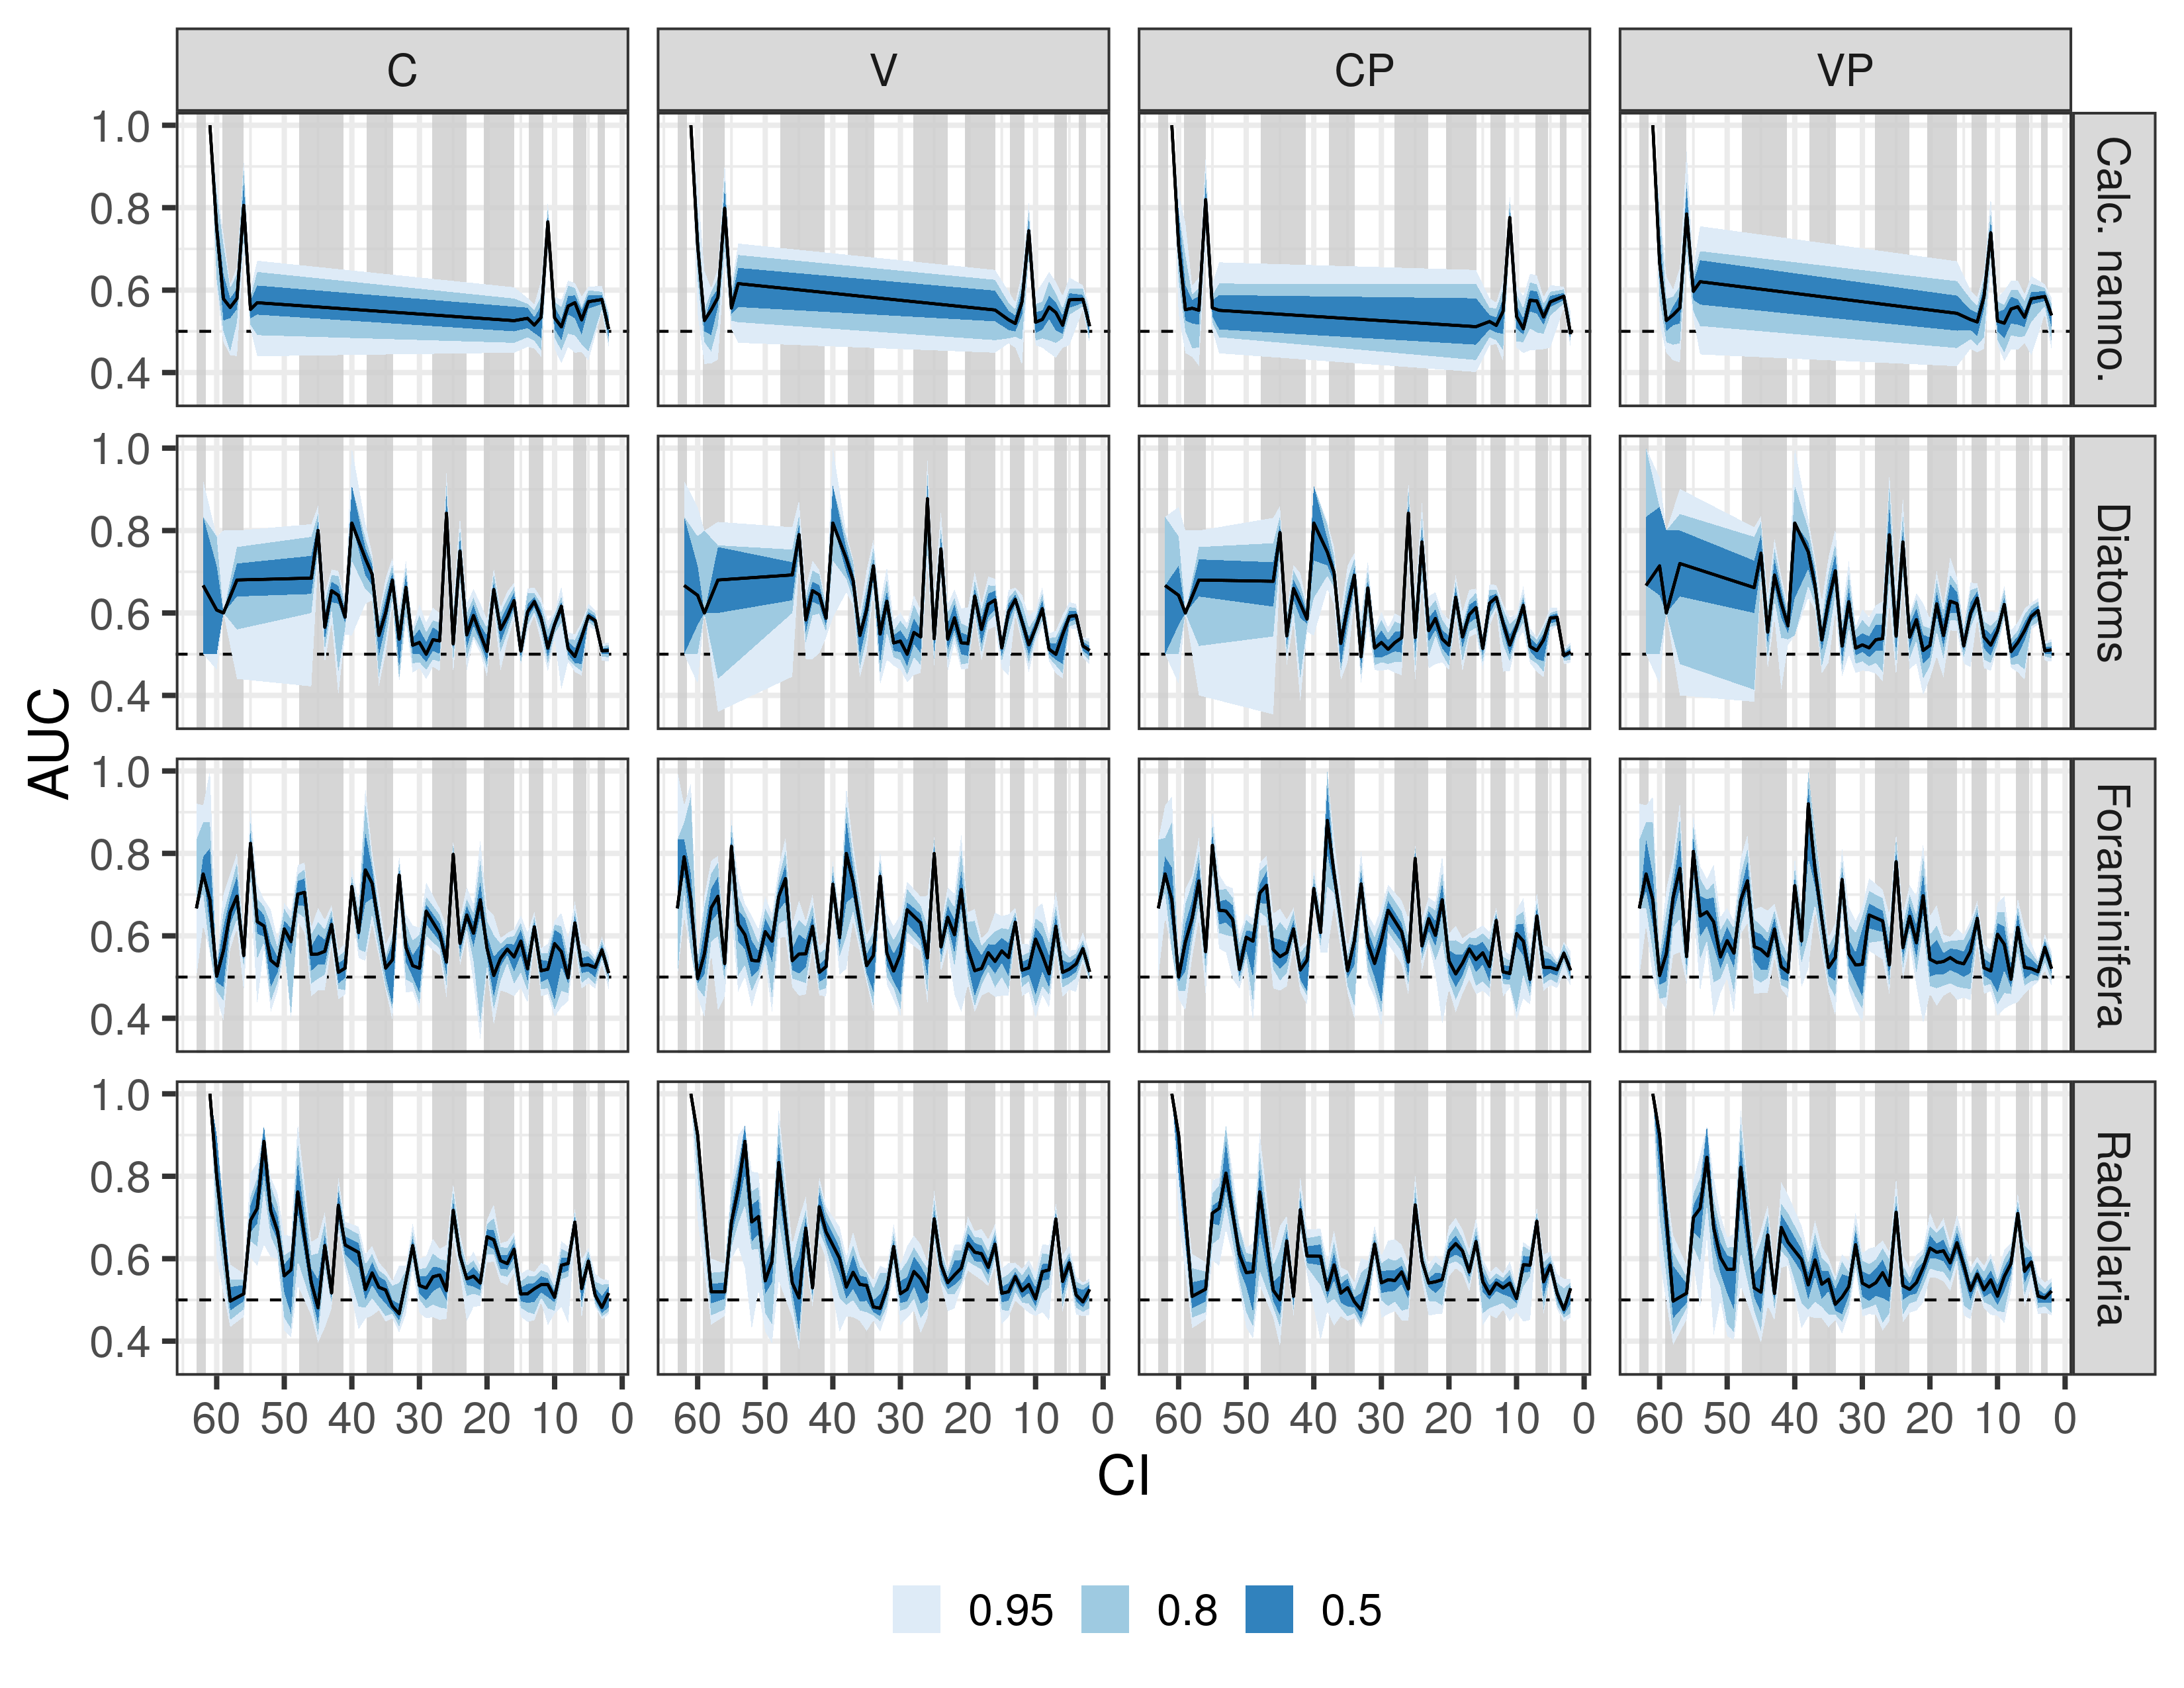
\includegraphics[width=\textwidth,height=0.5\textheight,keepaspectratio=true]{../results/figure/auc_taxon_time_full}
  \caption{Comparison of posterior predictive AUC estimates for each of the four models, arranged over time and by taxonomic group. These estimates reflect each model's fit to the various taxonomic groups over time. The black line corresponds to the median AUC value, while the envelopes correspond to multiple credible intervals as indicated in the legend. In all cases, higher AUC values indicate greater predictive performance versus lower AUC values. See Table \ref{tab:model_def} for a description of each of the four models.}
  \label{fig:auc_taxon_time}
\end{figure}




\subsection{Cross-validation}

Expected out-of-sample predictive performance was estimated using five-fold cross-validation, modified for time series data \citep{ESL}. This procedure yields four posterior (predictive) distributions, each corresponding to AUC values calculated from model-based predictions compared to the extinction state of the hold-out data. These four posterior predictive distributions are pooled to yield a posterior predictive distribution of expected out-of-sample performance -- the resulting distributions tend to be very multimodal due to their very nature being fit to and estimated from different data sets and amounts of data \citep{ESL}. Additionally, multimodality increases with model complexity (Fig. \ref{fig:fold_auc}) -- this makes sense as the more complex models allow for predictor effects to vary with time, allowing for a greater range in possible parameter values which in turn yield a greater range of posterior predictions.

Comparison between the posterior predictive distributions of expected out-of-sample AUC (Fig. \ref{fig:fold_auc}) reveals a similar range in plausible values for all models as the in-sample AUC posterior predictive distributions (Fig. \ref{fig:auc_hist}). Interestingly, the differences between the posterior predictive distributions for the models have decreased. For example, model VP not clearly better than either models V or CP (Fig. \ref{fig:fold_auc}), which were shown earlier to be obviously worse-performing models based on in-sample performance (Fig. \ref{fig:auc_hist}). These differences means that the rank order of median out-of-sample AUC is different from the rank order of median in-sample AUC. However, the shapes of the posterior distributions means interepting from the median values is incorrect -- the models are effectively indistinguishable in their expected out-of-sample AUC values.

Additionally, the quality of expected out-of-sample performance is not great, with average out-of-sample AUC for each of our models estimated to be between 0.7 and 0.8 which is far from perfect. This result means that we would expect to correctly rank two species in order of most to least likely to go extinct 70-80\% of the time. However, this expected out-of-sample performance is approximately the same as the in-sample performance results (Fig. \ref{fig:auc_hist}), indicating that our models would yield consistent results when generalized to future extinctions.

%When the posterior predictive distribution of expected out-of-sample AUC is presented as a time series, the similarity between the models is even more apparent (Fig. \ref{fig:fold_auc_time}). While the width of the credible intervals at various time points varies between the models, the overall picture of expected out-of-sample AUC is almost identical when you compare the models -- periods of relatively better or worse performance map identically between the time series.
%\begin{figure}[ht]
%  \centering
%  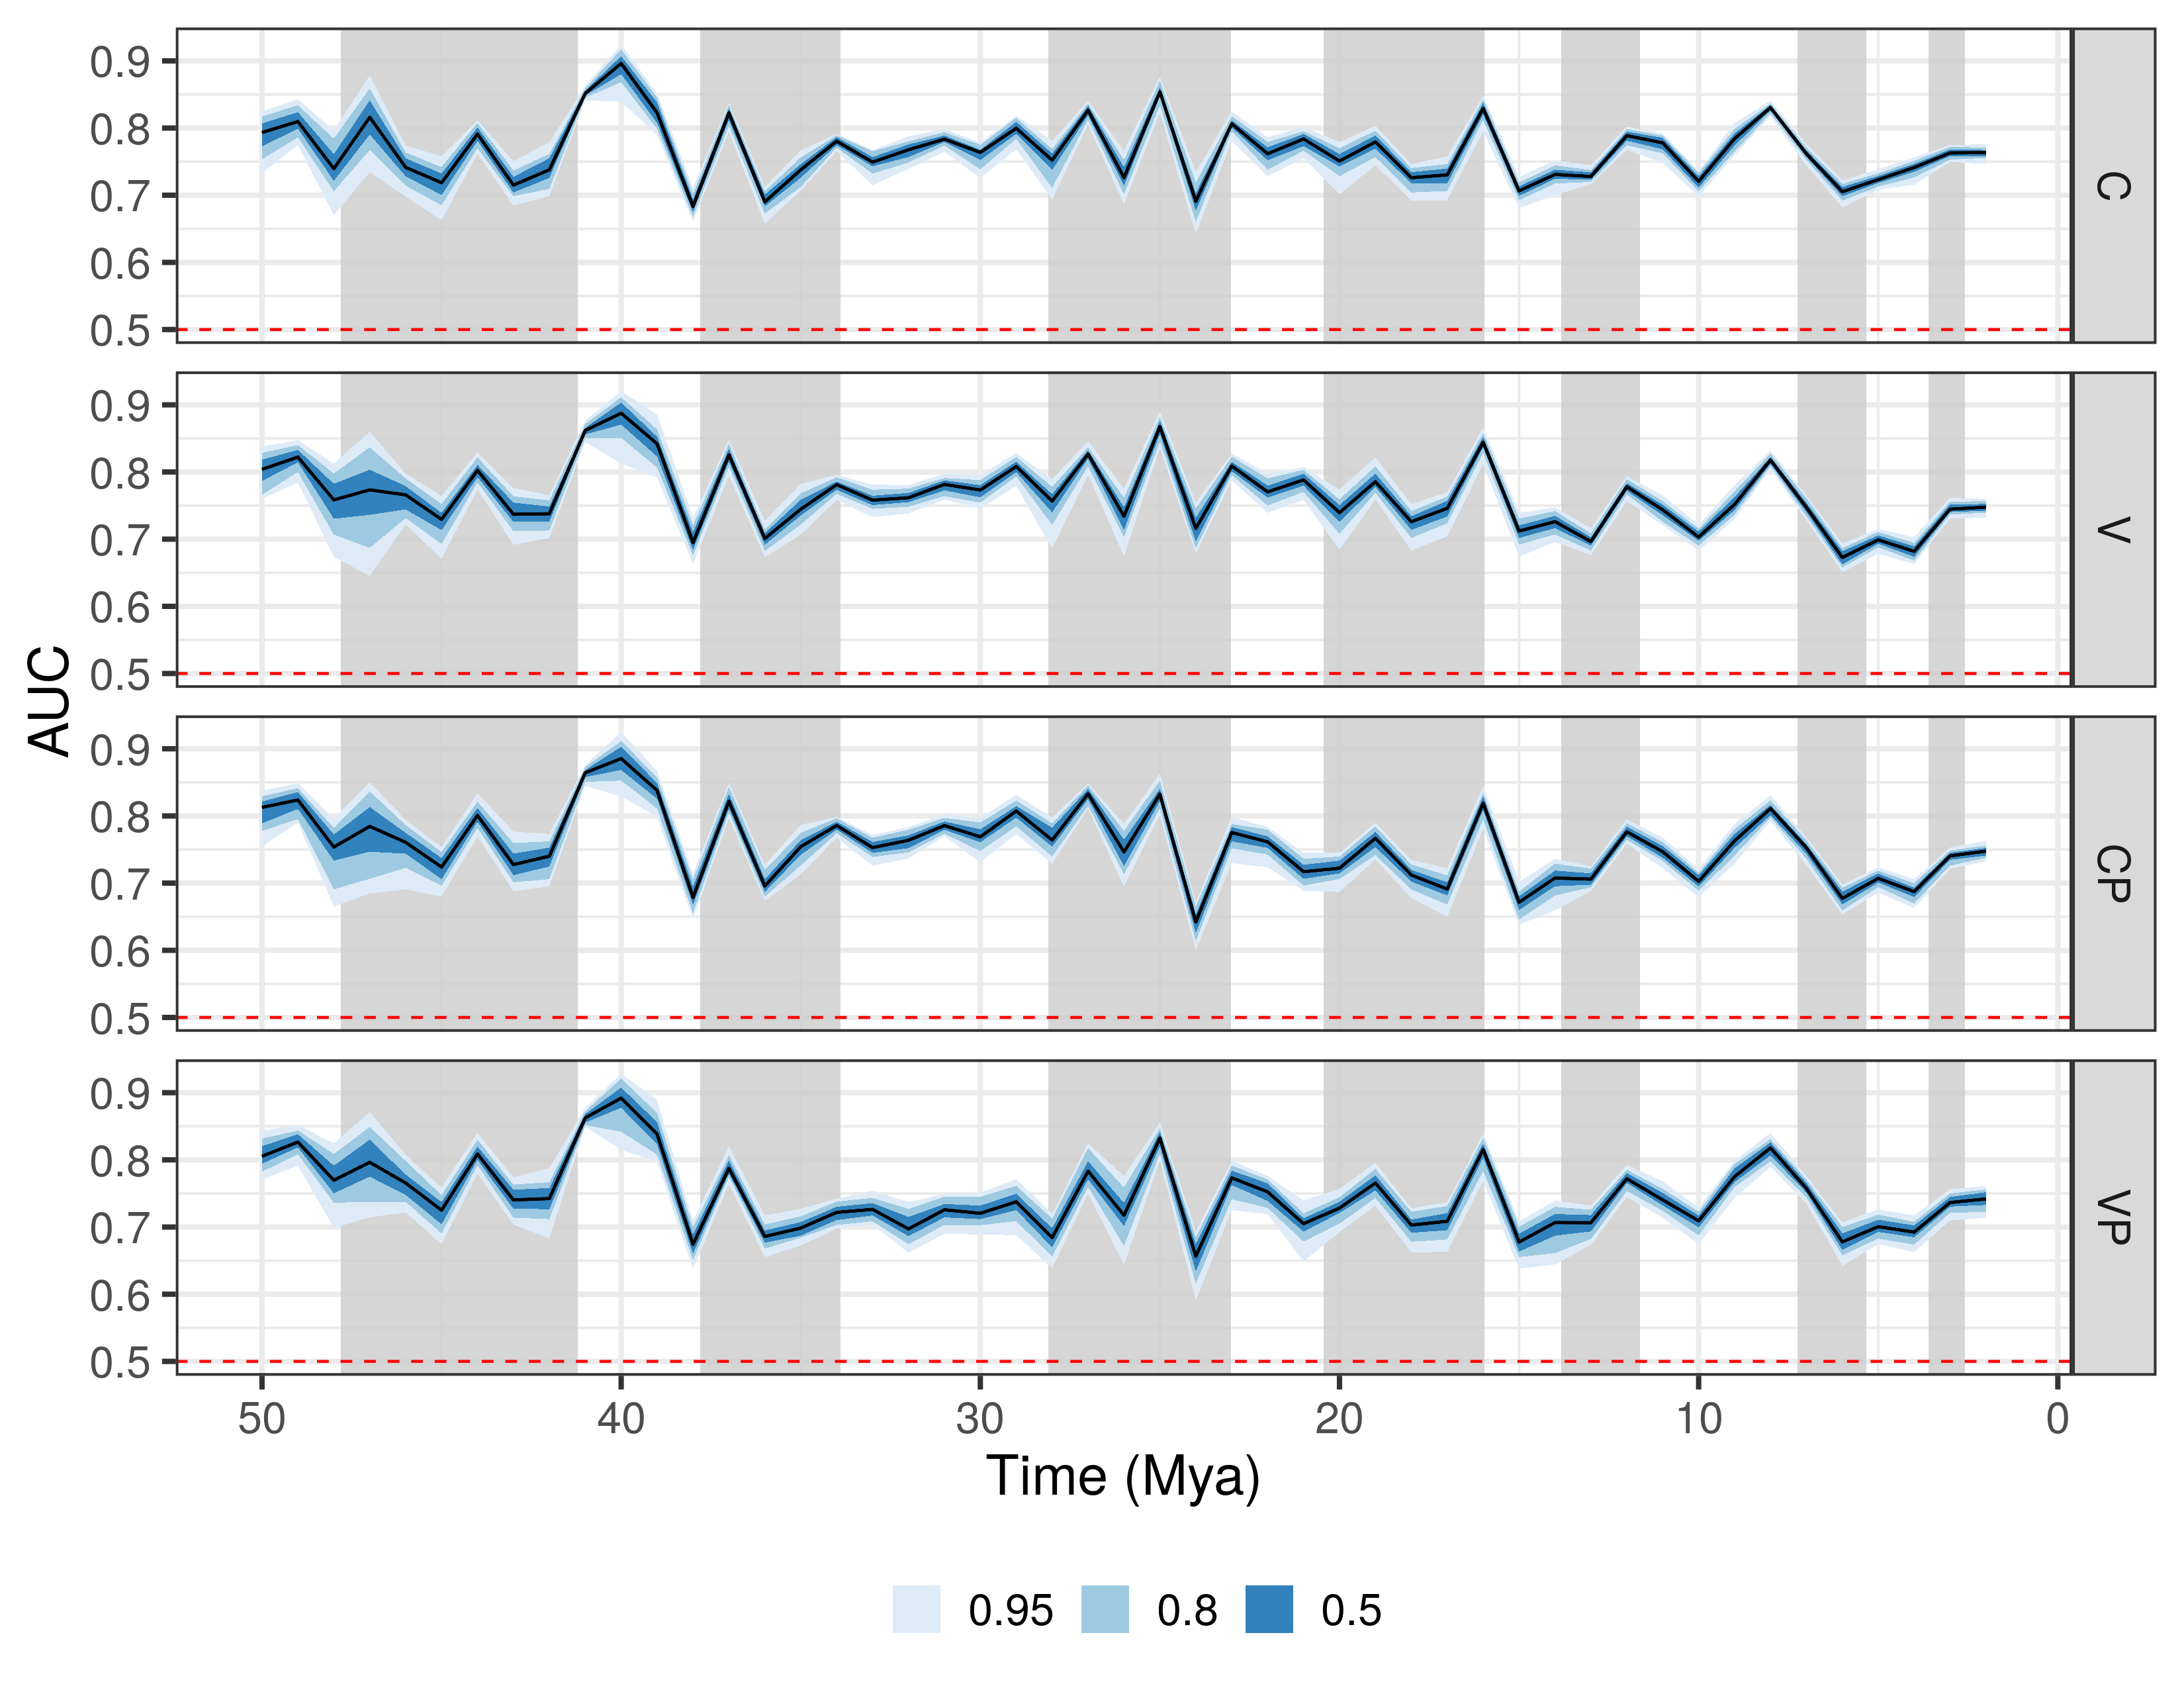
\includegraphics[width=\textwidth,height=0.5\textheight,keepaspectratio=true]{../results/figure/fold_auc_time_full}
%  \caption{Comparison of out-of-sample AUC values calculated for each of the My intervals for each of the four models. The AUC of the individual My intervals within each fold is plotted to highlight the heterogentity in performance within and between folds. This presentation decomposes each of the 12-million year folds (Fig. \ref{fig:fold_auc}) into the predictions made for each of the million-year intervals. The red line corresponds to the median AUC estimate, with the envelopes corresponding to multiple credible intervals as indicated in the legend.}
%  \label{fig:fold_auc_time}
%\end{figure}
%We can also compare expected out-of-sample AUC by taxonomic group for each of the models (Fig. \ref{fig:fold_auc_taxon}). These comparisons reveal a lot about the differences in predictive potential of the taxonomic groups. For example, the posterior predictive distributions of out-of-sample AUC for Foraminifera from all four models are approximately identical. In contrast, expected out-of-sample AUC for Radiolaria exhibits the same or similar pattern in relative model performance to the pooled comparisons (Fig. \ref{fig:fold_auc}). Additionally, we can state that our out-of-sample predictions for calcareous nannoplankton and dinoflagellates are not necessarily as precise as our estimates for Foraminifera or even Radiolaria. These results indicate that out-of-sample predictions may be easier for some taxonomic groups than others (e.g. Foraminifera versus Dinoflagellates.
%\begin{figure}[ht]
%  \centering
%  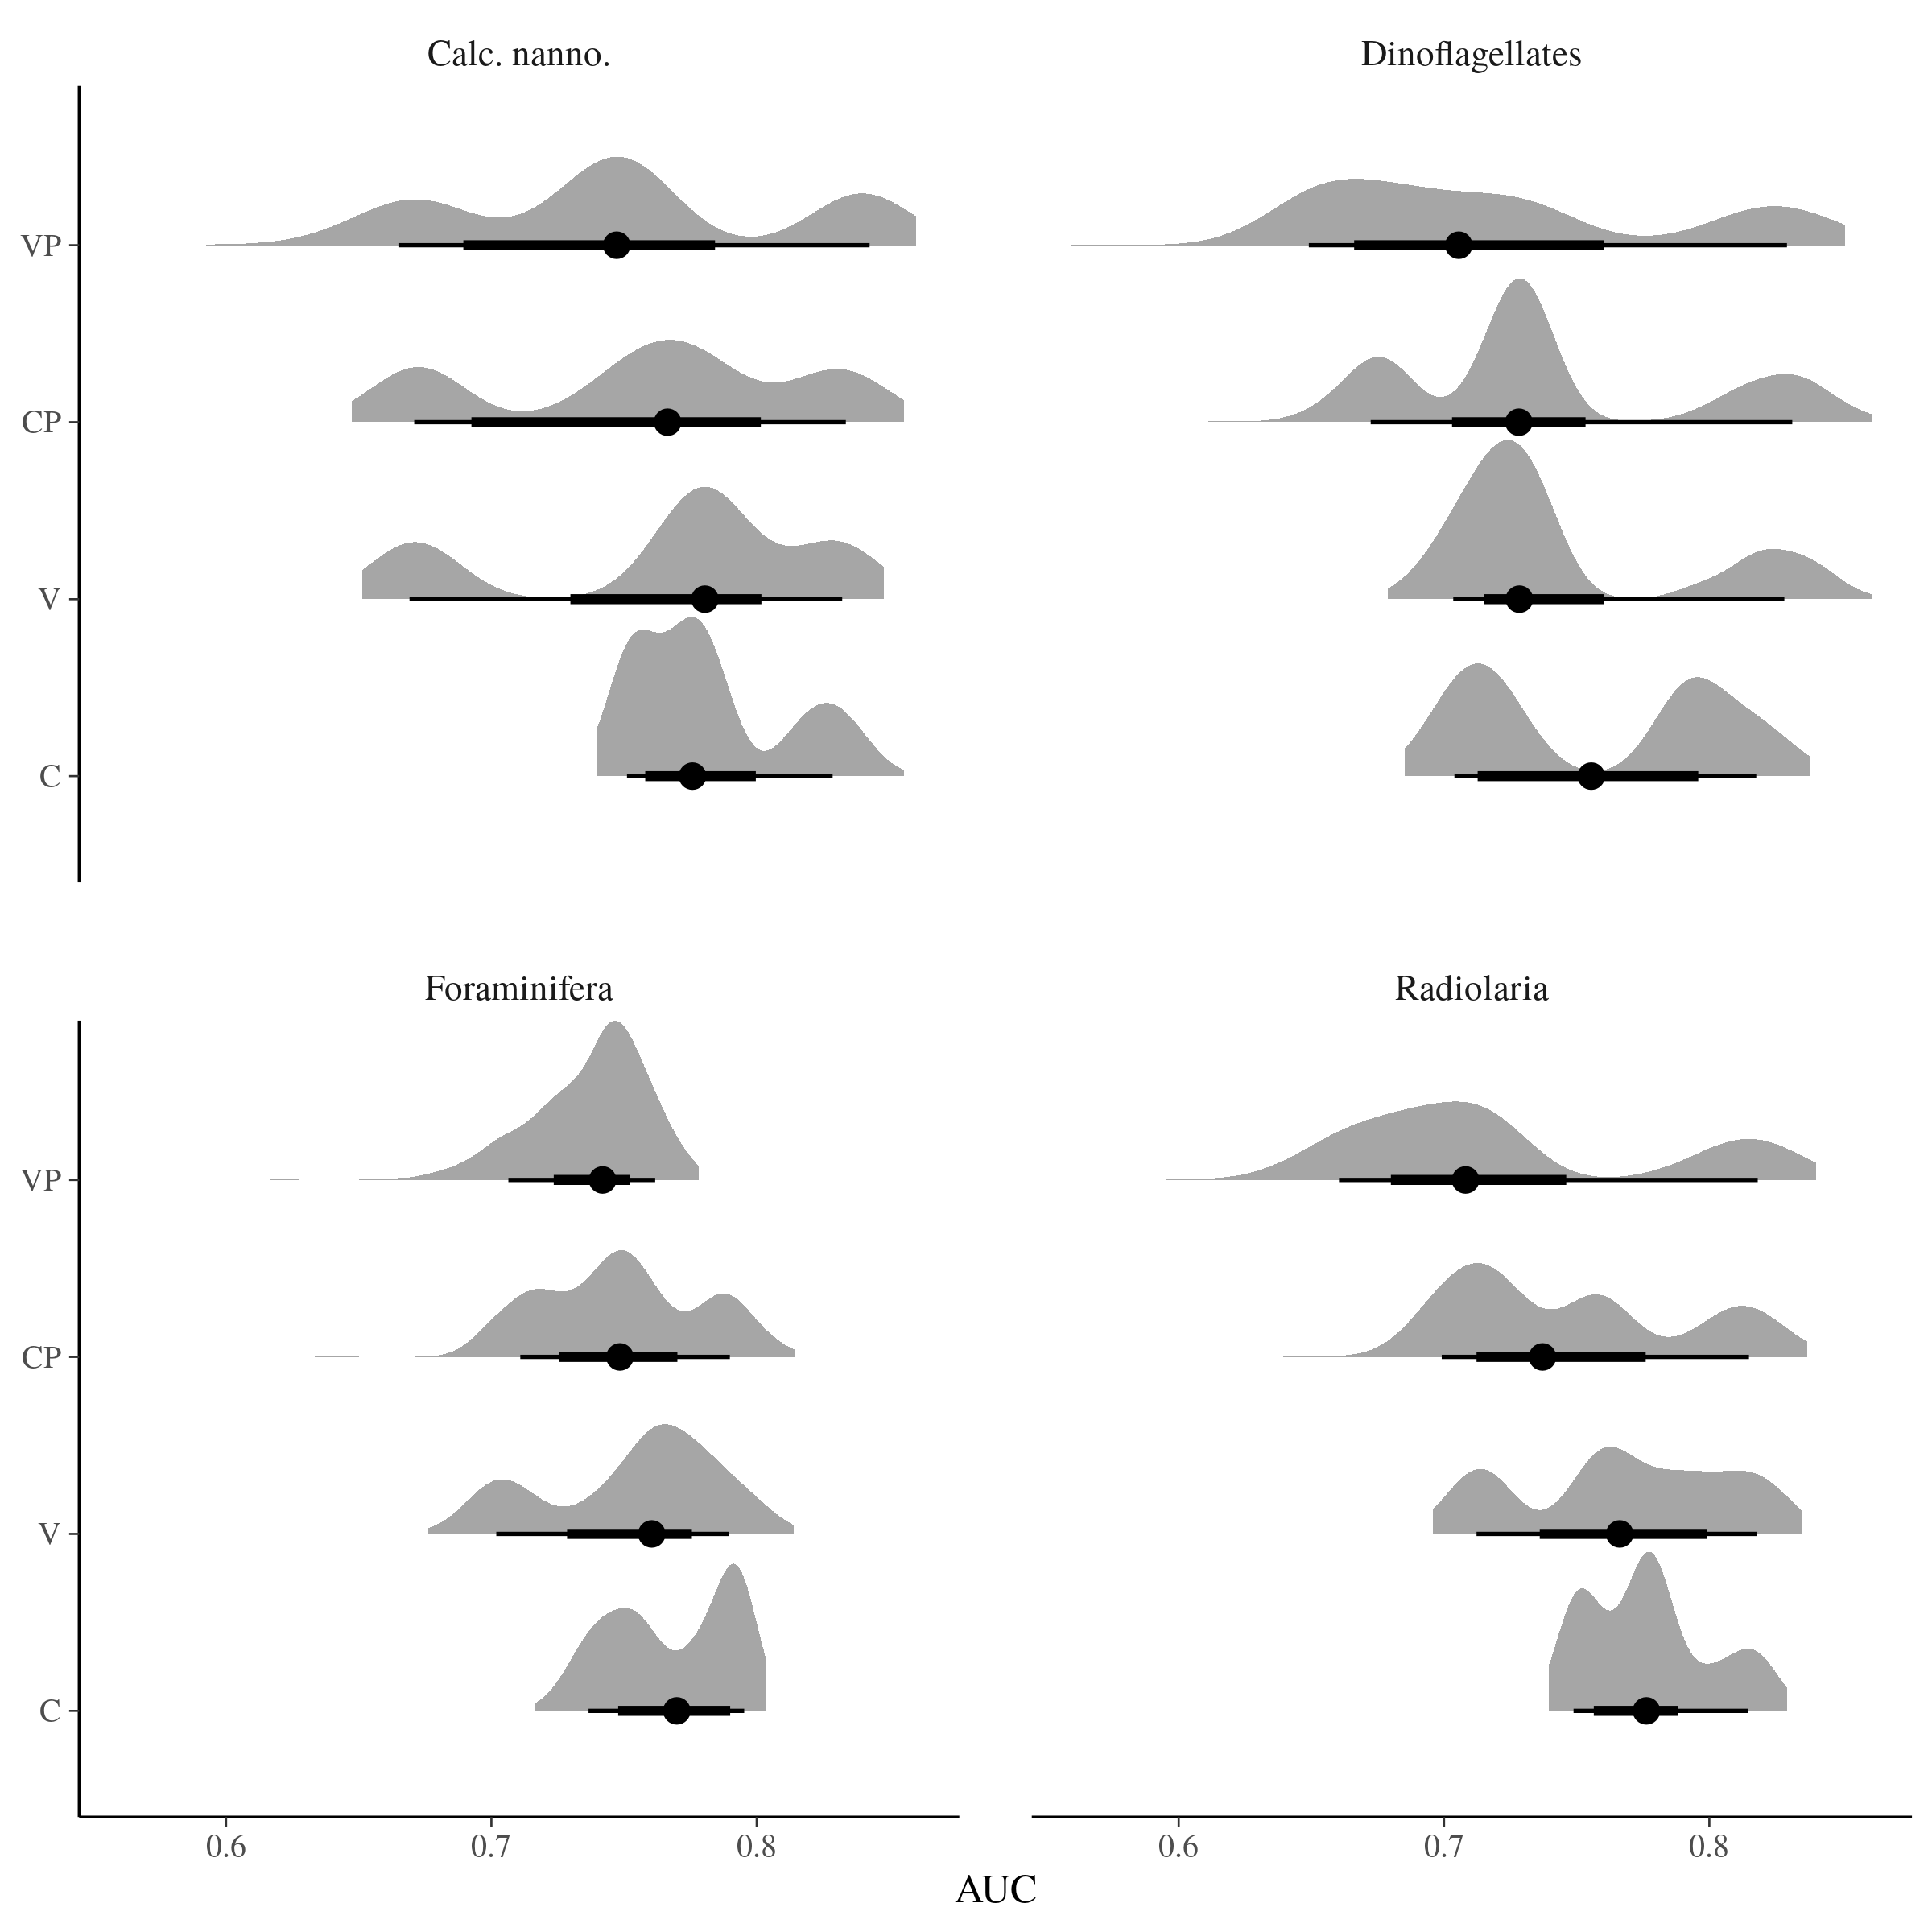
\includegraphics[width=\textwidth,height=0.5\textheight,keepaspectratio=true]{../results/figure/fold_auc_taxon_full}
%  \caption{Comparison of out-of-sample AUC values aggregated by taxonomic group for each of the four models. Depicted for each taxon-model combination is an aggregate density of all posterior predictive estimates for each of four folds -- cross-validation estimates are commonly multi-modal as each fold presents its own challenges for prediction. Beneath these densities is marked the median estimate along with 50\% and 80\% credible intervals.}
%  \label{fig:fold_auc_taxon}
%\end{figure}
%

We can also compare the posterior predictive distribution of expected out-of-sample AUC over time and taxonomic group for each of the four models (Fig. \ref{fig:fold_auc_taxon_time}). For each taxonomic group, the time-series of posterior predictive values for each model are broadly congruent. 

In the analysis of the posterior predictive distributions of the in-sample AUC values for the four models, we noted that there were time intervals where the models' predictions were no better than random (Fig. \ref{fig:auc_taxon_time}). This occurrence is generally much rarer for the posterior predictive distribution of out-of-sample AUC values -- the major exception to this is Dinoflagellates, which for all four models has at least one time interval where the median the AUC of out-of-sample data were no better random. In contrast, the only other group for which median posterior predictive estimate of out-of-sample AUC reaches 0.5 is calcareous nannoplankton, and then only with model V.
\begin{figure}[ht]
  \centering
  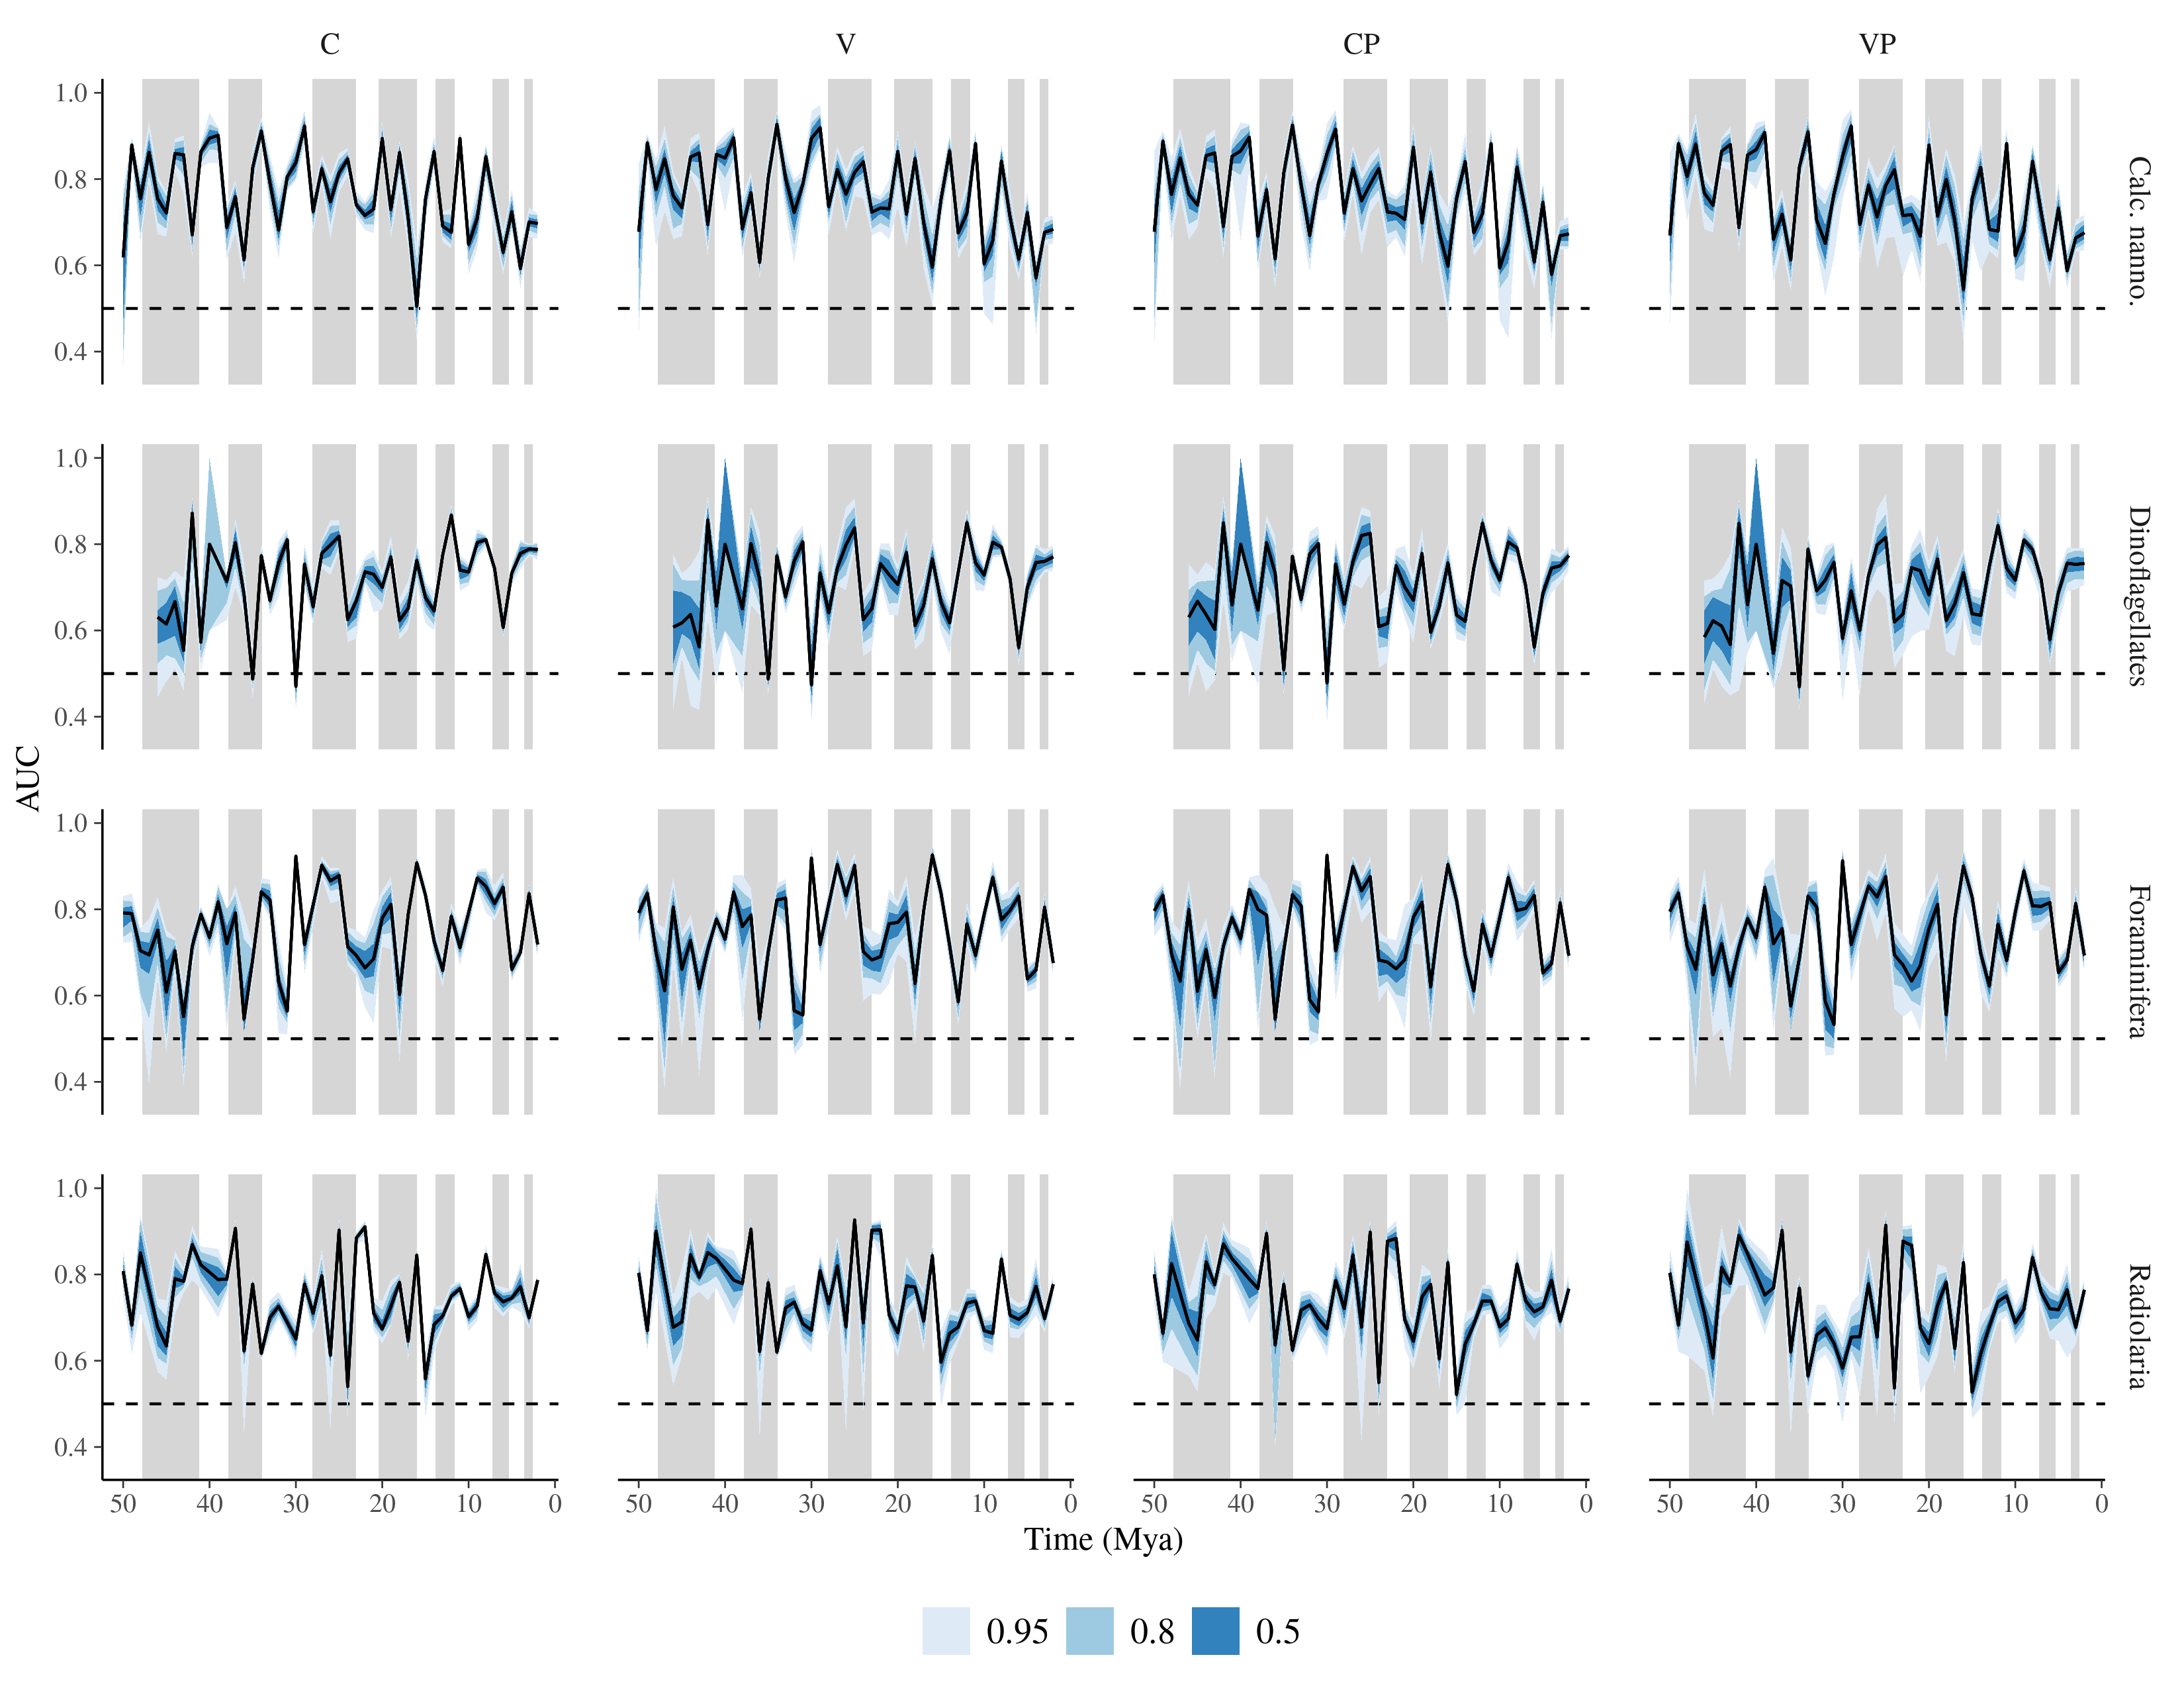
\includegraphics[width=\textwidth,height=0.5\textheight,keepaspectratio=true]{../results/figure/fold_auc_taxon_time_full}
  \caption{Comparison of out-of-sample AUC values over time as aggregated by taxonomic group for each of the four models. The AUC of the individual My intervals within each fold is plotted to highlight the heterogentity in performance within and between folds. This presentation decomposes each of the 12-million year folds by each of the taxonomic groups into the predictions made for each of the million-year intervals. The black line corresponds to the median AUC estimate, with the envelopes corresponding to multiple credible intervals as indicated in the legend. See Table \ref{tab:model_def} for a description of each of the four models.}
  \label{fig:fold_auc_taxon_time}
\end{figure}


%Looking at four randomly sampled species, we evaluated their probability of extinction at all times that species was observed. We then compared these estimates to the geographic range trajectory of 
%
%
%% risk estimate compared to change in geo-range
%\begin{figure}[ht]
%  \centering
%  \begin{subfigure}{\textwidth}
%    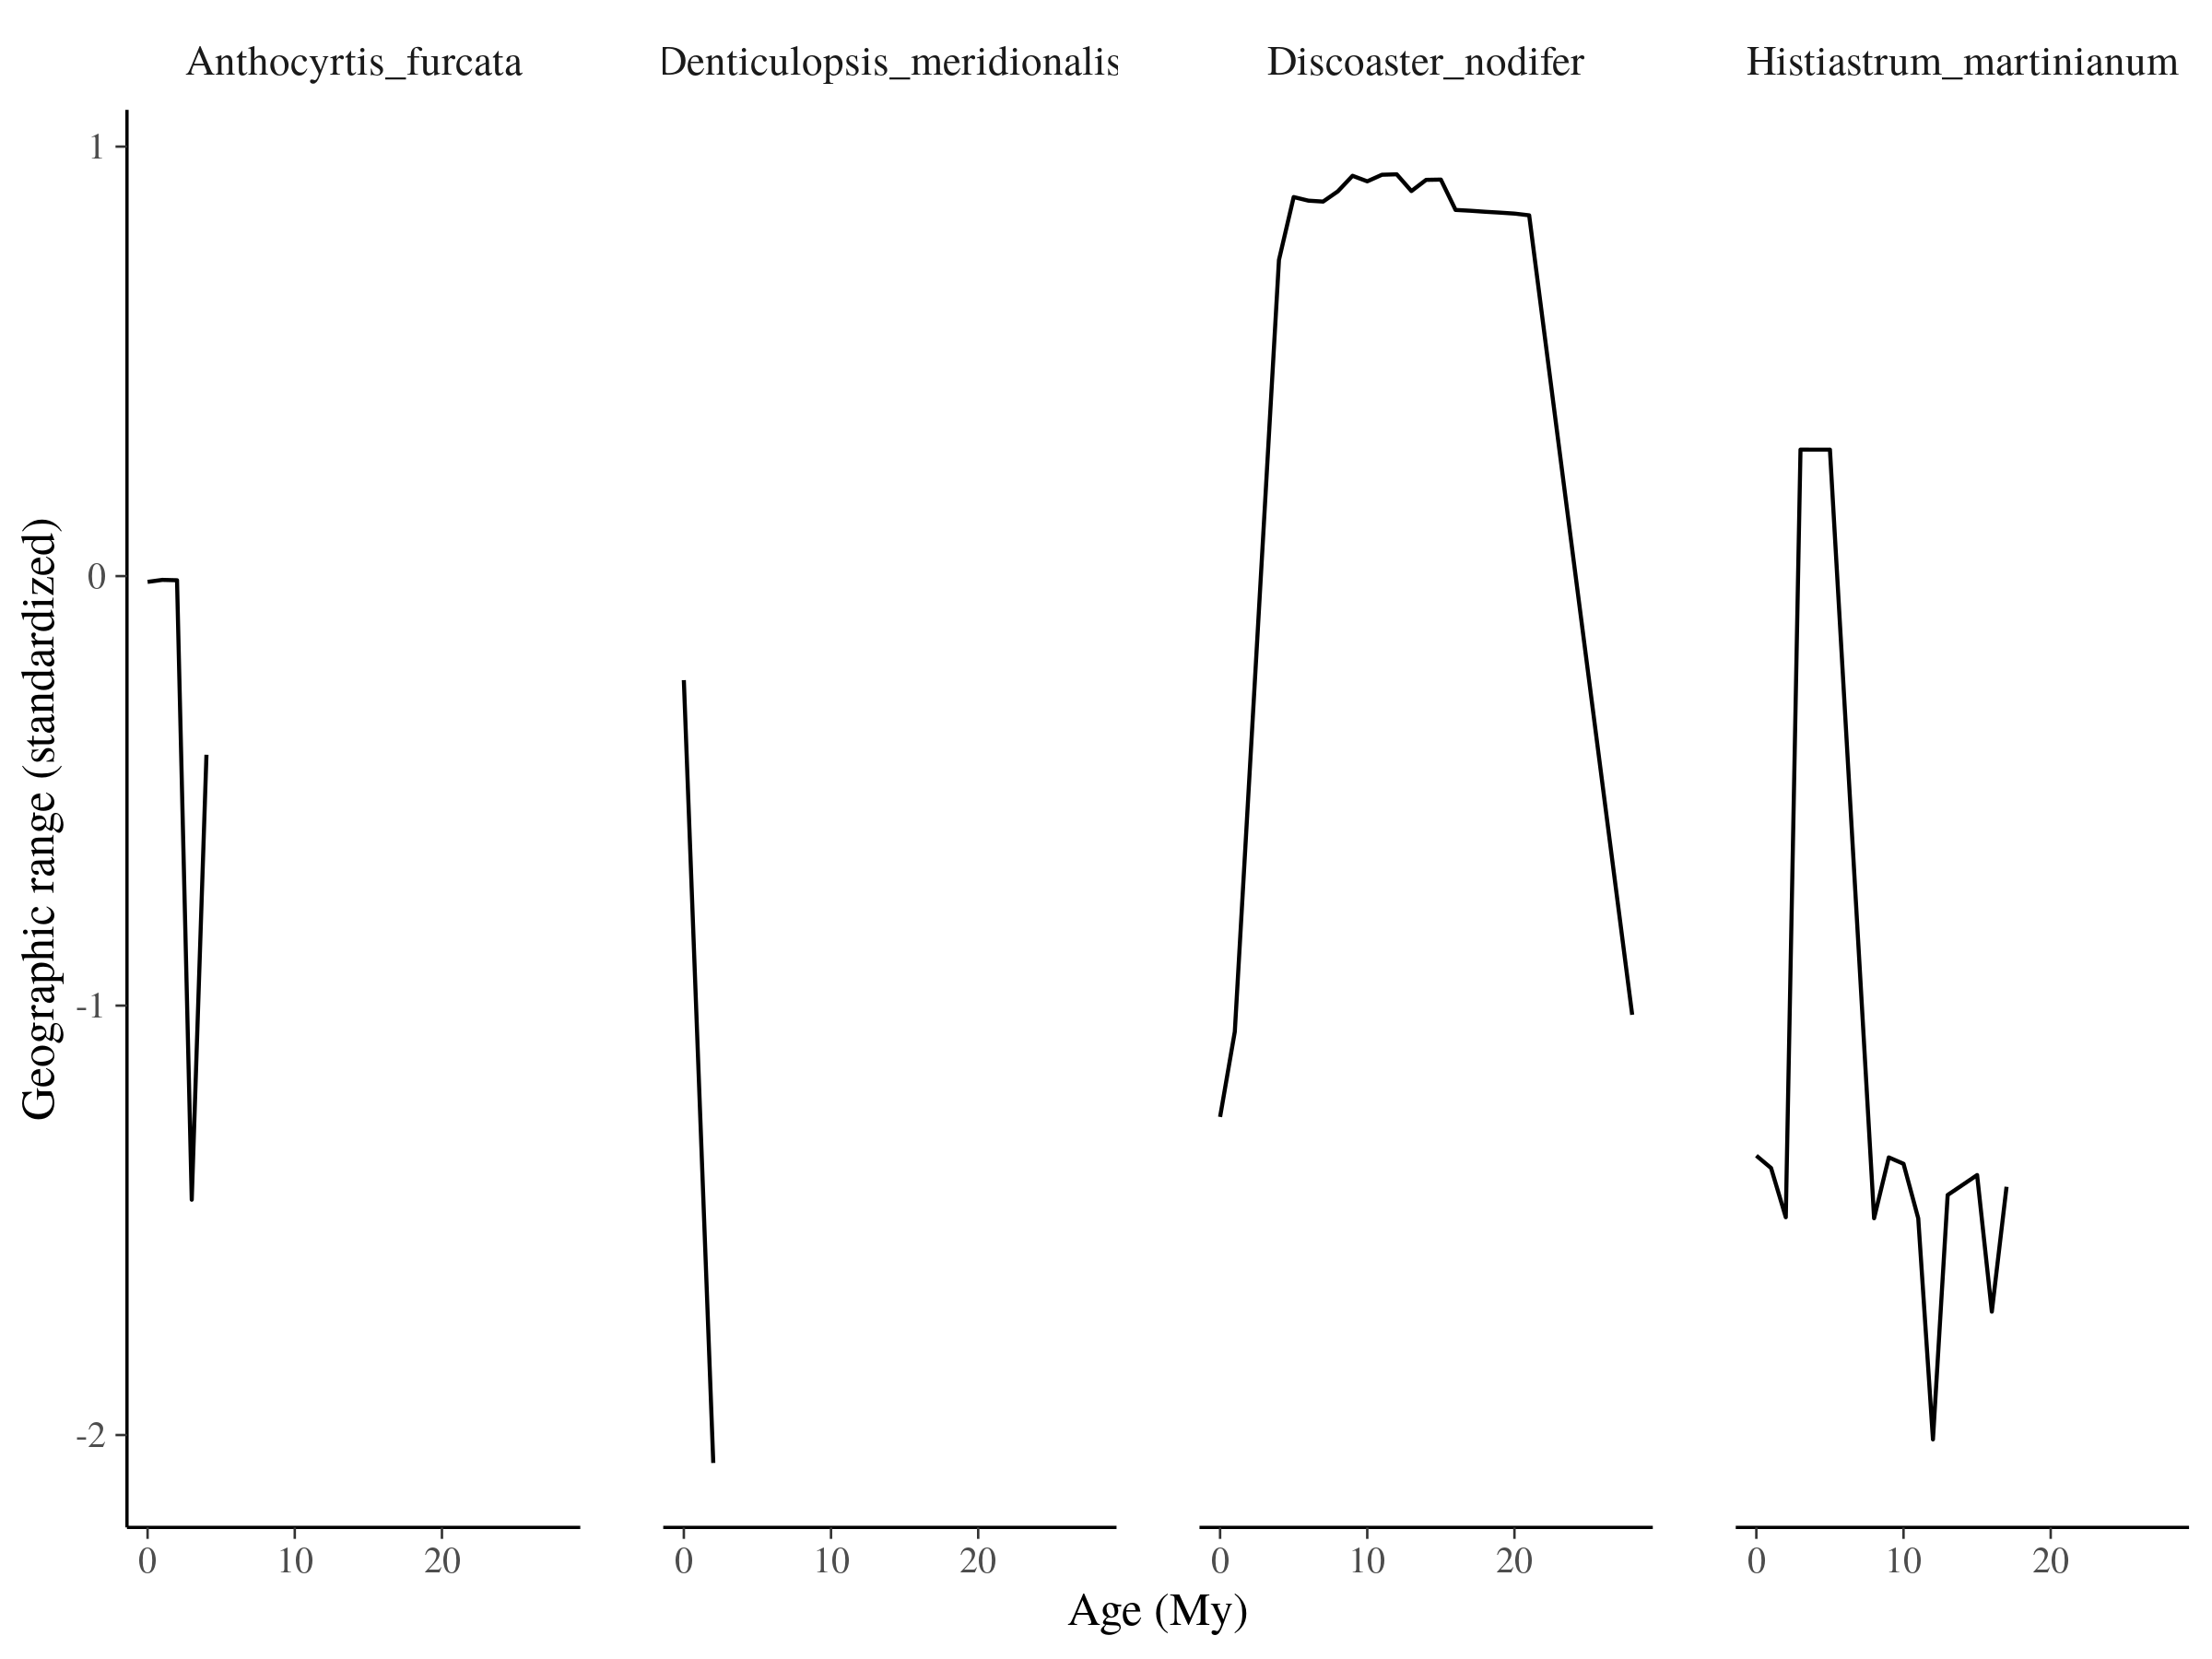
\includegraphics[width=\textwidth,height=0.5\textheight,keepaspectratio=true]{../results/figure/relrisk_range}
%    \caption{A}
%    \label{fig:relrisk_range}
%  \end{subfigure}
%
%  \begin{subfigure}{\textwidth}
%    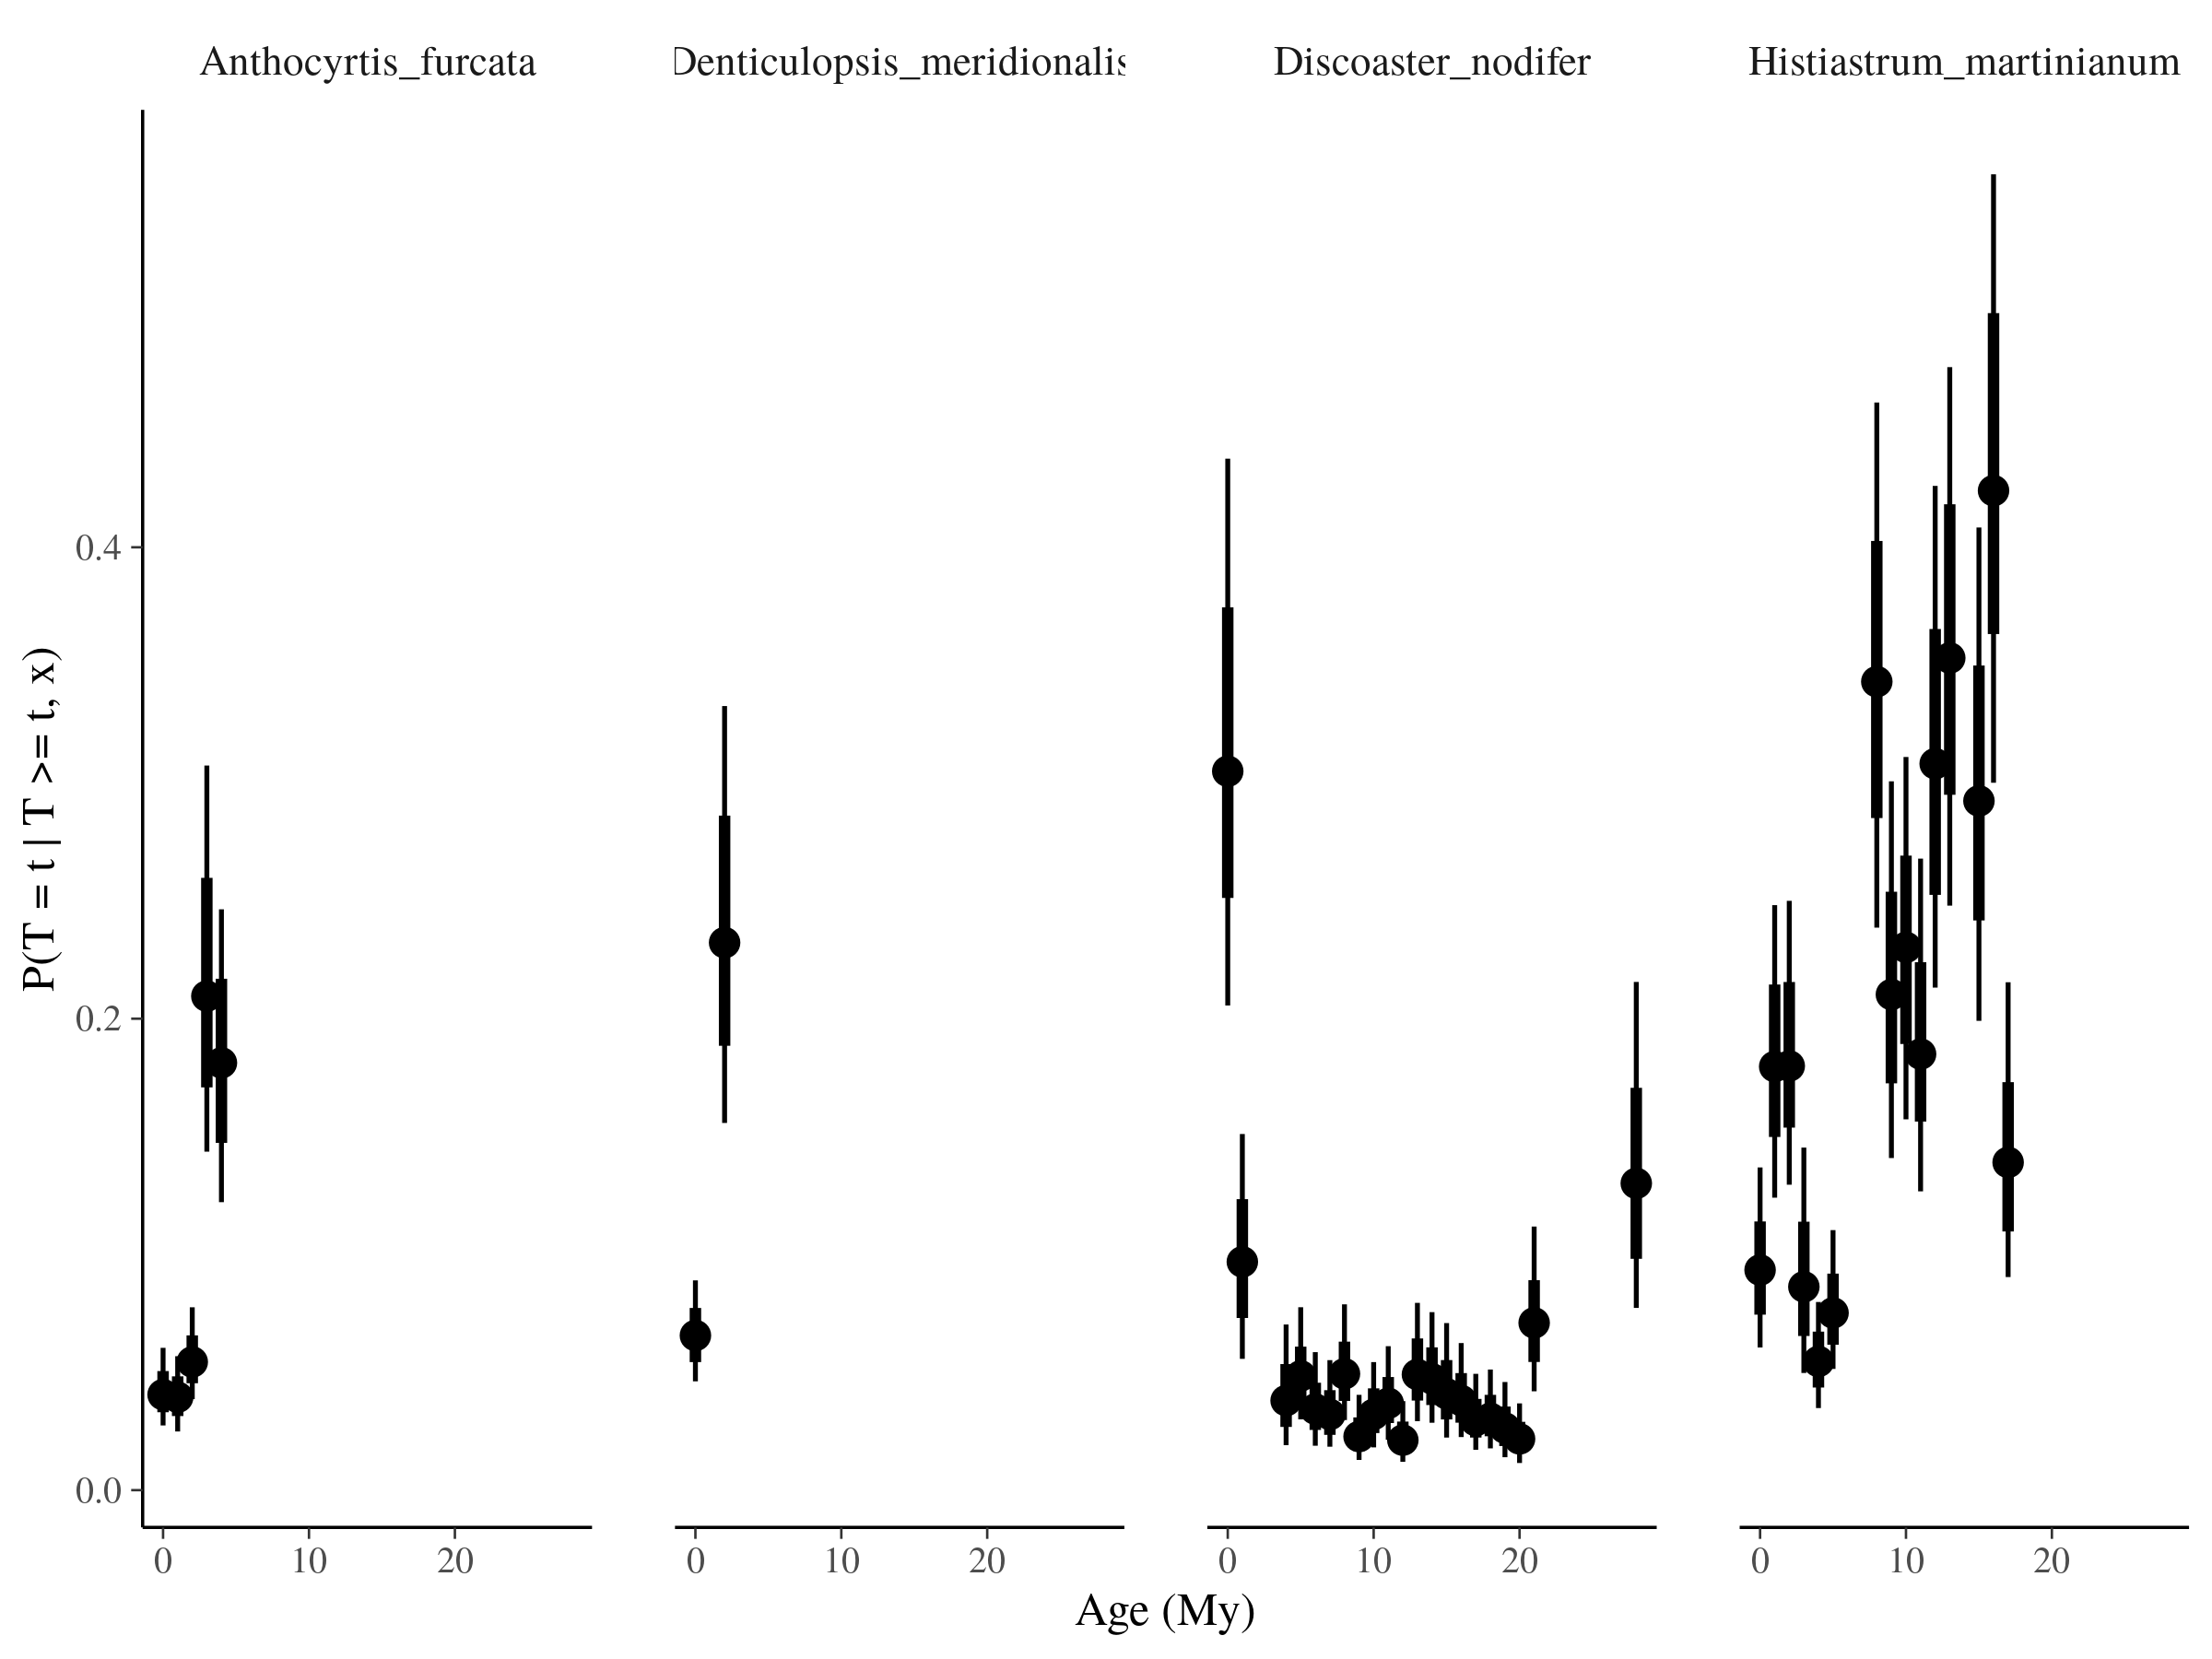
\includegraphics[width=\textwidth,height=0.5\textheight,keepaspectratio=true]{../results/figure/relrisk_ext}
%    \caption{B}
%    \label{fig:relrisk_ext}
%  \end{subfigure}
%  \caption{Comparison between species geogrpahic range histories and our estimate of their probability of extinction for each time of observation. Geographic range is assumed observed without error. Our probability estimates are presented as a median (point) and 50\% and 80\% credible intervals.}
%  \label{fig:relrisk_compare}
%\end{figure}



\section{Discussion}

The results of this paper set out our baseline ability to predict relative differences in extinction risk. We find that all of our model have an approximate 77\% to 79\% probability of correctly rank the extinction risk of two randomly selected in-sample observations. Similarly, these models are expected to correctly rank the extinction risk of two randomly selected out-of-sample observations approximately 70\% to 80\% of the time. A slight decrease in performance when dealing with out-of-sample observations makes sense: each of the models fit during cross-validation is based on less data than the model fit on the full data (between 1/5th to 4/5ths of the original). The similarly between the in-sample and out-of-sample results indicates that our model is fairly robust to how extinction intensity has changed over the Cenozoic.

One of the most striking results of this analysis is that the in-sample and out-of-sample comparisons between our models demonstrate that while models where the historical coarviates are predictors of species extinction have better in-sample performance (Fig. \ref{fig:auc_hist}, \ref{fig:auc_taxon_time}), all of them generalize to out-of-sample data with a similar degree of success (Fig. \ref{fig:fold_auc}, \ref{fig:fold_auc_taxon_time}).

Other noteworthy aspects of our in-sample results are that AUC estimates for our models models differ significantly between models and that all of these estimates are in a narrow range of possible AUC values (Fig. \ref{fig:auc_hist}). For our in-sample results, while the statistically best model does include the historical covariates and allows all covariate effects to vary over time, its practical difference in performance compared to the other models is virtually negligible (Fig. \ref{fig:fold_auc}). This means that even though model VP has a \textit{statistically} greater AUC than the other three models, this result is not practically or \textit{scientifically} significant. 

This result is an important reminder about understanding the practical interpretation of our analyses, which can be lost when we do not consider the predictive aspects of our analyses. By focusing on determining which covariates are ``significant'' and which model is best through simple comparisons means that the practical importance of the results are ignored. For example, in logistic regression a covariate can be considered significant on the log-odds scale but have no practical difference on the probability scale because the range of values is too small as to matter such as when the intercept is greater than 2 or less than -2 because the inverse-logit of those values are close to 0 or 1, respectively \citep{ARM}.

The success of model is partially driven by the size of our dataset and the hierarchical structure of our model. Our estimates are based on rather limited information about the taxa themselves, and our model only takes into account some aspects of species geographic range and their rough taxonomic grouping. Instead of relying on large amounts of ecological information to shape individual differences, our model leverages most of the Neptune dataset through a multilevel model to constrain and improve our parameter estimates by sharing information about those parameters across taxa and time.

The principal reason we were not able to include more biological information in our models is that we lack most any life history or ecological information on most marine micro- and nano-plankton. Forams are the exception to this problem -- there is life history, ecological, and physiological information for a selection of foram species \citep{Ezard2011}. However, not this information does not exist all foram species. If we want to include this type of information in a predictive model of extinction risk, we would be able to analyze only a single taxonomic subset of the fossil occurrences present the Neptune Database and then only a limited selection of those species. This means ignoring the majority of occurrence information present in the Neptune database.

This presents an interesting conundrum about how to improve upon our results. A simple hypothesis for how to improve upon our results is that if we were to include more biological information in our model, our estimates of species relative extinction risk would be improved. However, if we decrease the amount of data in our model, our results by definition decrease in their quality. For example, compare the results from our models fit using full in-sample dataset, and the results from the cross-validation where the fit to each fold is by definition based on less than full information.)



In conclusion, our results provide a promising picture of our ability to predict the relative extinction risk of two randomly selected species. Considering that conservation decisions are made based on a continuum of risk, from most to least, this means that our results are in the same language as how conservation resources are allocated.


% bibliographic information
\bibliographystyle{abbrvnat}
\bibliography{citations}



\section{Supplementary Material}
\beginsupplement

\subsection{Model Specifications} \label{sec:model_desc}

In survival analysis, the hazard function describes the instantaneous rate of extinction of a species given its age and relevant covariates. The hazard function is defined as the conditional probability of a species going extinct by the end of the \(t\)-th interval given that it survived up until \(t\) and the relevant covariate information \(X\) for all \(k\) 1 My intervals \citep{Tutz2016}. For the discrete time intervals \(T = 1, \cdots, k\), extinction is defined as \(T = t\). The discrete time hazard function is defined as
\begin{equation}
  \lambda(t | X) = P(T = t | T \geq t, X), \quad t = 1, \cdots, k.
  \label{eq:hazard}
\end{equation}

The hazard function (Eq. \ref{eq:hazard}) is easily reparameterized as a logistic regression by defining that \(\lambda(t | X) = h(\Theta)\) where \(h(.)\) is a logit inverse-link function and \(\Theta\) is the probability of a taxon going extinction during interval \(t\) \citep{Tutz2016}. \(h(\Theta)\) is then modeled as with any regression as it is defined for all real-values. In this case, we opted for a hierarchical/mixed-effects model with multiple non-nested varying intercepts and slopes \citep{ARM}.

Our covariates matrix \(X\) is a \(N \times D\) matrix where \(N\) is the total number of observations and \(D\) is the total number of covariates. The first column of \(X\) is entirely 1's as it corresponds to the intercept term in the regression model. The next two columns of \(X\) are two aspects of geographic range as continuous covariates: geographic range \(r\) during interval \(t\), and the difference \(d\) between the geographic range at \(t - 1\) and \(t\). The difference in geographic range was calculated from the transformed and standardized geographic range values; this means that change in geographic range is in units of changes in standard deviations. The final two columns are two aspects of global temperature: mean temperature during interval \(t\), and the lag of mean temperature (i.e. mean temperature during interval \(t - 1\).) As with change to geographic range, the lag of temperature is based on the transformed and standardized temperature estimates. 

The matrix of time and phylum varying regression coefficients describing the effects of the covariates on a species' risk of extinction is called \(B\) -- a  \(w\) by \(p\) matrix, were \(w\) is the number of time temporal intervals and \(p\) is the number of phyla. The elements of this matrix, the regression coefficients, are themselves modeled as being multivariate normally distributed with vector of means \(\alpha\) describing the average intercept and regression coefficient estimates of each coefficients for each phylum \(p\). These phylum averages are themselves modeled as multivariate normally distributed with mean vector \(\mu\) describing the overall average regression coefficients, including the intercept. \(\mu\) has length \(D\) and is ordered intercept, range coefficient, change in range coefficient, temperature coefficient, temperature lag coefficient.

The effect of species age on the log-odds of species extinction is modeled as a non-nested random intercept \(A\) \citep{Tutz2016}. This term describes how the log-odds of extinction varies along a species duration, and how this effect can differ between the phyla. \(A\) is a \(l\) by \(p\) matrix, where \(l\) is the age at observation of a species and \(p\) is its phylum. \(A\) is modeled as following a multivariate normal distribution with phylum means being vector \(\delta\) and covariance matrix \(\Sigma_{A}\). The covariation between the elements of vector \(\delta\) are modeled as a multivariate normal distribution with a mean vector of all 0s and covariance matrix \(\Sigma_{\delta}\).

To complete the generative model, we need to assign final priors to the ``top level'' parameters. In general we favored weakly informative priors which help regularize our estimates. In the case of a regression coefficient, this means a Normal distribution with mean 0 and a standard deviation of 3. For our scale parameters (e.g. standard deviations), we used half-Cauchy distributed priors with heavy tails but the majority of probability density near 0.

Our top-level intercept was given a more diffuse prior than our regression coefficients, which reflects our greater degree of uncertainty about its value. Our top-level regression coefficient for the effect of geographic range was given an informative prior reflecting the overwhelming amount of evidence that species with a larger than average geographic range have a lower risk of extinction than species with an average or less than average geographic range. In the context of this analysis, this means that we are again using a weakly informative prior but instead of centering the density around -1 (i.e. larger than average geographic range decreases extinction risk).

Instead of assigning a prior distribution for each of the covariance matrices in the model, we instead decomposed the covariance matrices (e.g. \(\Sigma_{B}\)) which allows us to assign independent priors for the scale and correlation aspects of covariance. The scale parameters were assigned half-Cauchy priors as described above in the context of all other scale parameters. The correlation matrices were assigned LKJ priors each with shape parameter set to 1. This choice of shape parameter produces a uniform distribution over possible correlation matrices. These priors are also slightly more interpretable than other common prior distributions for covariance matrices such as the inverse-Wishart distribution. This approach to assigning priors to a covariance matrix is recommended by the Stan Manual \citep{StanManual}.

In total, our model can be expressed as: 
\begin{equation}
  \begin{aligned}
    t_{i} &\sim \text{Bernoulli}(\Theta) \\
    \Theta_{i} &= \text{logit}^{-1} (X_{i} B_{w[i], p[i]} + A_{l[i], p[i]}) \\
    B_{w, p} &\sim MVN(\alpha_{p}, \Sigma_{B}) \\
    \alpha_{p} &\sim MVN(\mu, \Sigma_{\alpha}) \\
    % double check this\dots is A MVN dist?
    A_{l, p} &\sim MVN(\delta_{p}, \Sigma_{A}) \\
    \delta_{p} &\sim \mathrm{N}(0, \sigma_{\delta}) \\
    \mu_{d} &\sim 
    \begin{cases}
      N(-2, 5) & \text{if } d = \text{intercept} \\
      N(-1, 1) & \text{if } d = \text{geo. range} \\
      N(0, 1) & \text{else } \\
    \end{cases} \\
    \delta &\sim N(0, 1) \\
    \Sigma_{B} &= diag(\tau_{B}) \Omega_{B} diag(\tau_{B}) \\
    \Sigma_{\alpha} &= diag(\tau_{\alpha}) \Omega_{\alpha} diag(\tau_{\alpha}) \\
    \Sigma_{A} &= diag(\tau_{A}) \Omega_{A} diag(\tau_{A}) \\
    \tau_{B} &\sim C^{+}(1) \\
    \tau_{\alpha} &\sim C^{+}(1) \\
    \tau_{A} &\sim C^{+}(1) \\
    \Omega_{B} &\sim LKJ(1) \\
    \Omega_{\alpha} &\sim LKJ(1) \\
    \Omega_{A} &\sim LKJ(1) \\
  \end{aligned}
  \label{eq:model}
\end{equation}
with \(i\) indexing the observation and bracket subscripts referencing the class of the \(i\)th observation where \(w[i]\) is the time of the \(i\)-th observation, \(p[i]\) is the phylum of the \(i\)-th observation, and \(d[i]\) is the age of the \(i\)-th observation. 



\subsection{Model Parameter Estimation} \label{sec:model_est}

We implemented our model (Eq. \ref{eq:model} using the \begin{texttt}rstanarm\end{texttt} package for the R programming language \citep{StanManual}. This package provides an interface to the Stan probabilistic programming language for writing hierarchical/mixed-effects models in native R. Posterior estimates were obtained through Hamiltonian Monte Carlo, using 2000 steps divided equally between warm-up and sampling. In order to prevent divergent transitions the adapt delta value was increased to 0.9999; all other HMC/NUTS sampling parameters were kept at the defaults for rstanarm 2.18.2 \citep{rstanarm}.

An implementation of our full model in \begin{texttt}rstanarm\end{texttt}, given a data.frame of all necessary data in a data.frame called ``data'', is coded as:
\begin{verbatim}
form <- event ~ range + range_diff + temp + temp_lag + 
                (1 + range + range_diff + temp + temp_lag | mybin/phylum) + 
                (1 | age/phylum), 
stan_glmer(formula = form,
           data = data, 
           family = 'binomial',
           prior = normal(c(-1, 0, 0, 0), rep(1, 4), autoscale = FALSE), 
           prior_intercept = normal(-2, 5, autoscale = FALSE), 
           prior_aux = cauchy(0, 1, autoscale = FALSE), 
           chains = 4,
           thin = 4,
           adapt_delta = 0.999999)
\end{verbatim}

Similarly, our full model can also be implemented using the \begin{texttt}brms\end{texttt} Stan interface \citep{brms2017,brms2018} as:
\begin{verbatim}
priors <- c(set_prior('normal(-2, 5)', class= 'Intercept'),
            set_prior('normal(0, 1)', class = 'b'),
            set_prior('normal(-1, 1)', class = 'b', coef = 'range'),
            set_prior('cauchy(0, 1)', class = 'sd'),
            set_prior('lkj(1)', class = 'cor'))
form <- bf(event ~ range + range_diff + temp + temp_lag +
           (1 + range + range_diff + temp + temp_lag | mybin/phylum) +
           (1 | age/phylum))
brmfit <- brm(formula = form,
              data = data, 
              family = bernoulli(), 
              prior = priors,
              chains = 4, 
              thin = 4,
              control = list(adapt_delta = 0.999999)
\end{verbatim}

Posterior convergence was determined using the general and HMC-specific diagnostic criteria: scale reduction factor (\(\hat{R}\); target \(<1.1\)), effective sample size (eff; target value eff/steps \(<0.0001\)), number of samples that saturated the maximum trajectory length for avoiding infinite loops (treedepth; target value 0), sample divergence, and the energy Bayesian Fraction of Mission Information (E-BFMI; target value \(>0.2\)). For further explanation of these diagnostic criteria, see the Stan Manual \citep{StanManual}.




\end{document}
